 % PRB regular article source -- channel-projected surgical revision
\documentclass[%
  aps,prb,reprint,amsmath,amssymb,superscriptaddress,longbibliography,floatfix
]{revtex4-2}

\usepackage{graphicx}
\usepackage{dcolumn}
\usepackage{bm}
\usepackage{physics}
\usepackage{hyperref}
\hypersetup{hidelinks}
\usepackage{xcolor}
\usepackage{booktabs}
\usepackage{enumitem}
\usepackage[section]{placeins}
\usepackage{xr-hyper}

\newcommand{\PT}{\mathcal{PT}}
\newcommand{\Hss}{H_{\rm ss}}
\newcommand{\Htilde}{\tilde{H}}
\newcommand{\teps}{\tilde{\epsilon}_{\xi}}
\newcommand{\keff}{\kappa_{\rm imp}}
\newcommand{\Gless}{G^{<}}
\newcommand{\Gret}{G^{R}}
\newcommand{\Gadv}{G^{A}}
\newcommand{\tb}{\tilde{\beta}}          % gauge-invariant SBMF scale
\newcommand{\gb}{\beta_0}               % signed frozen drive-control amplitude
\newcommand{\gm}{\gamma}                % flip in frozen BA
\newcommand{\Gpt}{\Gamma_{\mathrm{PT}}}   % projected gain/loss channel
\newcommand{\dSig}{\delta_{\Sigma}}          % real one-body self-energy shift
\newcommand{\Deff}{\Delta_{\rm eff}}     % projected coherent splitting/flip
\newcommand{\Dzero}{\Delta_0}              % static coherent splitting in generic projection
\newcommand{\Dcoh}{\Delta_{\rm coh}}          % Kramers--Kronig coherent detuning
\newcommand{\Veff}{V_{\rm eff}}           % projected impurity-bath hybridization
\newcommand{\cGm}{c_{\Gamma}}
\newcommand{\cDl}{c_{\Delta}}
\newcommand{\cV}{c_V}


\externaldocument[M-]{main}
\begin{document}
\title{Supplemental Material for ``Emergent $\PT$ Symmetry and Exceptional Points in a Driven Dirac Impurity''}
\author{Vinayak M.~Kulkarni}
\affiliation{Theoretical Sciences Unit,
  Jawaharlal Nehru Centre for Advanced Scientific Research,
  Bangalore 560064, India}
\date{\today}
\maketitle

This Supplemental Material provides the technical derivations and validation
checks that support the self-contained main article.  It includes the
auxiliary-mode influence functional, Keldysh mean-field equations, physical-FDR
construction, number continuity, shifted-resonance condition, the complete
biorthogonal and finite-$U$ charge resolvents, one-particle scattering-phase
checks, the controlled branchwise linearization, the exact finite-$U$
two-electron contact algebra, and numerical validation figures.

\section*{Notation and parameter conventions}
\begin{description}[leftmargin=1.6cm,style=nextline]
\item[$t_{\rm av},\tau,T_{\rm b}$]
Wigner center time $(t+t')/2$, relative time $t-t'$, and reservoir temperature.
\item[$\eta,\zeta_\sigma$]
Chiral bath index $\eta=\pm$ and spin sign $\zeta_\uparrow=+1$, $\zeta_\downarrow=-1$.
\item[$\lambda,j_\alpha$]
SOC strength and eigenvalues of the dimensionless exchange matrix $\rho_bJ^{\rm bio}$; $j_{\rm scr}$ is the largest positive real part.
\item[$\alpha_{\rm b},k_{\rm max},D_{\rm uv}$]
Quadratic bath-dispersion coefficient, radial momentum cutoff, and ultraviolet energy cutoff.  The two cutoffs are set numerically to $\pi/4$ in the dimensionless plots but are not the same physical quantity.
\item[$W_k,W,\Lambda_\eta^{\rm PV}$]
Static bare impurity--bath hybridization and principal-value bath shift.
The drive does not set $W_k$; at the saddle the vertex is $rW_k$.
\item[$\beta_0,\tilde\beta$]
Signed frozen drive-control amplitude and nonnegative SBMF projection
$\tilde\beta=|\beta_0||b_c|$.  The local core and the SOC-degenerate $k=0$
bath-dressed condition coincide exactly at
$\beta_{0,{\rm core}}^{\rm EP}=0.50$; the finite-$k$ operational
Schur-tracked minimum on the plotted path is
$\beta_{0,{\rm proj}}^{\rm min}=0.4975$.
\item[$s$]
Impurity pole splitting; $\zeta_\sigma$ is used for the spin sign.
\item[$\mathsf{s}_a,\delta_a$]
Eigenvalues $\mathsf{s}_a=e^{2i\delta_a}$ and eigenphases of the complete
unitary scattering matrix.  They are distinct from the EP pole splitting
$s$ and from the fixed chiral labels $\eta=\pm$.
\item[$\gamma,\Gamma_{\rm PT},\bar\Gamma$]
Bare coherent impurity flip, passive relative decay imbalance, and common bath width.  The symbols $\tilde\Gamma_\eta$ and $\Gamma_\sigma^{\rm net}$ denote, respectively, the chiral frozen-kernel width and the physical net channel width.
\item[$\omega,\Omega,\omega_0$]
Fourier frequency, drive frequency, and a selected spectral pole or resonance frequency; none of these denotes temperature.
\item[$\mathcal E_n,E_{\rm EP},\Lambda(\omega)$]
Non-Hermitian eigenvalues, EP eigenvalue, and real bath self-energy.
\item[$\mathcal P,\mathfrak a,\mathfrak b$]
Full-kernel Schur polynomial and the two local contact denominators; these are distinct from the bath coefficient $\alpha_{\rm b}$.
\item[$\mathcal F_{\rm dist},\mathcal F_{\rm MF}$]
Distribution matrix and mean-field free-energy functional.
\end{description}

\appendix
% ============================================================


\section{Impurity-block EP condition and condition-number scaling}
\label{app:harmonic}
\label{app:EP_scaling}

This appendix records the impurity-block algebra used in the main text.
The Hadamard rotation itself is shown in
Eqs.~(\ref{M-eq:imp_rotated})--(\ref{M-eq:V_rotated}); here we keep only
the EP and condition-number scaling that underlies the diagnostic
interpretation.

The frozen impurity block is
$h_d=\bigl[\begin{smallmatrix}\teps+\gm&i\gb\\i\gb&\teps-\gm
\end{smallmatrix}\bigr]$, with eigenvalues $E_\pm=\teps\pm s$
and splitting $s=\sqrt{\gm^2-\gb^2}$.  The regimes are
$\PT$-unbroken ($\gm>\gb$), exceptional ($\gm=\gb$), and
$\PT$-broken ($\gb>\gm$).  Right eigenvectors may be chosen as
$|r_\pm\rangle\propto[\gb,\,i(\gm\mp s)]^T$, so
\begin{equation}
\det R=2i\gb s,
\qquad R=(|r_+\rangle,|r_-\rangle).
\label{eq:detR}
\end{equation}
Thus, near the bare EP,
\begin{equation}
\keff=\|R\|\|R^{-1}\|\sim\frac{C}{|s|},
\label{eq:kappa_scaling}
\end{equation}
with a nonsingular constant $C$.  The standard local \(U\) does not cut off
this algebraic divergence on the equal-velocity, scalar-hybridization
linearized submanifold because it preserves the complexified pseudospin
symmetry.  Physical observables built from the complete resolvent remain
finite.  Curvature, unequal velocities, frequency dependence, or
component-dependent vertices can lift the exact symmetry and must be
analyzed separately.

\subsection{Slave-boson scaling and the core EP}

The bare impurity--bath hybridization $W$ in Eq.~(3) of the main article is
time independent.  At the saddle it becomes $rW$.  Since the projected
impurity self-energy is $\Sigma_d=W^\dagger G_cW$, every induced impurity
channel carries the same factor $r^2$:
\begin{equation}
\Gamma_{\rm PT}=r^2\Gamma_{\rm PT}^{(0)}(\beta_0),\quad
\Delta_{\rm eff}=r^2[\Delta_0^{(0)}+c_\Delta^{(0)}\beta_0],\quad
\bar\Gamma=r^2\Gamma_0 .
\label{eq:r2_channels}
\end{equation}
Consequently
\begin{equation}
h_{\rm rel}^2
=r^4\left\{[\Delta_0^{(0)}+c_\Delta^{(0)}\beta_0]^2
-[\Gamma_{\rm PT}^{(0)}(\beta_0)]^2\right\}I .
\label{eq:r4_identity_app}
\end{equation}
The common $r^4$ cancels from the local core condition for every $r>0$.
At $r=0$ the result is an ordinary decoupled degeneracy.  A bath-dressed
finite-$k$ minimum can drift because the SOC-resolved Schur terms do not
remain a common scalar shift; it must be tracked separately.
At $k=0$, by contrast,
$\varepsilon_{c,+}(0)=\varepsilon_{c,-}(0)=0$, and the Schur polynomial
factorizes exactly as
\begin{align}
\mathcal P(z,0)
&=\left(z-\tilde\epsilon_\xi-\frac{r^2W^2}{z}\right)^2
\nonumber\\[-0.2em]
&\quad-r^4\!\left\{[\Delta_0^{(0)}+c_\Delta^{(0)}\beta_0]^2
-[\Gamma_{\rm PT}^{(0)}(\beta_0)]^2\right\}.
\label{eq:k0_factorization_app}
\end{align}
The impurity-related $k=0$ double-root condition is therefore exactly the
local core condition for arbitrary $W$ and $r>0$.

\section{Angular Harmonic Decomposition and 2D$\to$1D Reduction}
\label{app:angular}

We show how the 2D Dirac bath with trigonal anisotropy reduces to
an effective 1D problem after integrating out all angular-momentum
harmonics $m\neq0$.
This Gaussian reduction is the microscopic origin of the
1D BA structure in Sec.~\ref{M-sec:BA}.

\subsection{Angular Fourier Decomposition}

In 2D polar momentum coordinates $(k,\theta)$, the bath fermion
is decomposed into angular-momentum channels:
\begin{equation}
c_{k,\theta,\sigma}
=\frac{1}{\sqrt{2\pi}}\sum_{m=-\infty}^{\infty}
c_{k,m,\sigma}\,e^{im\theta}.
\label{eq:ang_decomp}
\end{equation}
The impurity at position $\mathbf{r}=0$ (the lattice site) is local,
so only the isotropic ($m=0$) channel hybridizes with it:
\begin{equation}
c_{\mathbf{r}=0,\sigma}
=\sum_k\frac{1}{\sqrt{2\pi}}\,c_{k,0,\sigma}.
\label{eq:local_bath}
\end{equation}
Higher harmonics $m\neq0$ are decoupled from the impurity in
the absence of anisotropy.

\subsection{$C_3$ Selection Rule from $\cos3\theta$}

The trigonal anisotropy $\beta_3(k)k^3\cos3\theta$ is expanded as
$\cos3\theta=\frac{1}{2}(e^{3i\theta}+e^{-3i\theta})$.
Substituting Eq.~(\ref{eq:ang_decomp}) and performing the
$\theta$ integral:
$\int_0^{2\pi}\frac{d\theta}{2\pi}\,e^{i(m'-m)\theta}\,e^{\pm3i\theta}
=\delta_{m',m\mp3}$.
The trigonal term therefore couples only channels differing by
$\Delta m=\pm3$:
\begin{equation}
V_{\rm trig}\propto\sum_{k,\sigma,m}
c^\dagger_{k,m,\sigma}c_{k,m-3,\sigma}+\mathrm{h.c.}
\label{eq:Vselect}
\end{equation}
The auxiliary fermions $O_{k,m,\sigma}$ represent precisely the
$m=\pm3,\pm6,\ldots$ channels activated by this selection rule.


\subsection{Gaussian Integration and Passive Relative Kernel}

Since $H_O+H_{\rm hyb}$ is bilinear in $O_{k,m,\sigma}$, integrating out
all $m\neq0$ modes is a Gaussian path integral within the quadratic
auxiliary sector.  For fixed $(k,\theta,\sigma)$ the auxiliary action has
exactly the form
\begin{equation}
\begin{split}
S_O+S_{cO}=&
\int_{\mathcal C}dt dt'\,\bar O(t)A_O(t,t')O(t') \\
&+\int_{\mathcal C}dt\,
\left[\bar c(t)V_\sigma(t)O(t)
+\bar O(t)V_\sigma^\dagger(t)c(t)\right].
\end{split}
\label{eq:app_grassmann_action}
\end{equation}
The Grassmann integral gives the exact quadratic influence action
\begin{equation}
S_{\rm infl}
=-\int_{\mathcal C}dt dt'\,
\bar c(t)V_\sigma(t)g_O(t,t')V_\sigma^\dagger(t')c(t'),
\label{eq:app_influence_action}
\end{equation}
so the explicit retarded vertex contraction is
\begin{align}
\Sigma_\sigma^{O,R}(t,t')
&=\sum_{m,m'\neq0}
V_{m\sigma}(t)\,
 g_{mm'}^{O,R}(t,t')\,
V^*_{m'\sigma}(t') .
\label{eq:app_vertex_contraction}
\end{align}
No anomalous auxiliary propagator is used.  For a number-conserving
Hermitian auxiliary Hamiltonian this contraction contains the phase
difference fixed by the vertex and its Hermitian conjugate.  The Wigner
step connecting this two-time expression to the frozen bath self-energy can
be displayed explicitly.  Set $T=t_{\rm av}=(t+t')/2$ and $\tau=t-t'$, and
write $\mathcal V_{mm'}=V_mV_{m'}^*e^{i3(m-m')\theta}$.  To first adiabatic
order,
\begin{align}
&V_{m\sigma}(T+\tau/2)V_{m'\sigma}^*(T-\tau/2)
\notag\\
&\quad=\mathcal V_{mm'}
e^{i\zeta_\sigma[\phi(T+\tau/2)-\phi(T-\tau/2)]}
\notag\\
&\quad=\mathcal V_{mm'}e^{i\zeta_\sigma\tau\dot\phi(T)}
\left[1+O(\tau^3\partial_T^3\phi)\right].
\label{eq:app_wigner_phase}
\end{align}
For a stationary auxiliary propagator, its Wigner transform is consequently
\begin{align}
\Sigma_\sigma^{O,R}(\omega,T)
&=\Sigma_0^{O,R}[\omega+\zeta_\sigma\dot\phi(T)]
\notag\\
&=\Sigma_0^{O,R}(\omega)
+\zeta_\sigma\dot\phi(T)\partial_\omega\Sigma_0^{O,R}(\omega)
\notag\\
&\quad+O[(\Omega/\epsilon_O)^2].
\label{eq:app_wigner_shift}
\end{align}
Here the remainder denotes the relative gradient correction in the off-shell
window $|\omega-\epsilon_O^{(m)}|\sim\epsilon_O$.  Defining
\begin{equation}
\Sigma_0^{\rm bath,R}=\Sigma_{\rm bg}^R+\Sigma_0^{O,R},
\qquad
\Delta_{\rm aux}=\dot\phi(T)\partial_\omega
\operatorname{Re}\Sigma_0^{O,R},
\label{eq:app_aux_definitions}
\end{equation}
therefore gives
\begin{equation}
\begin{split}
\Sigma_{\sigma}^{\rm bath,R}(\omega,T)
=&\,\Sigma_0^{\rm bath,R}(\omega)
+\zeta_\sigma\Delta_{\rm aux}(\omega,T) \\
&+O[(\Omega/\epsilon_O)^2],
\qquad \Delta_{\rm aux}\in\mathbb{R} .
\end{split}
\label{eq:app_aux_shift}
\end{equation}
For diagonal remote modes,
\begin{align}
\Sigma_0^{O,R}(\omega)
&=\sum_{m\ne0}\frac{|V_m|^2}
{\omega-\epsilon_O^{(m)}+i0^+},
\notag\\
\Delta_{\rm aux}
&=-\dot\phi(T)\sum_{m\ne0}|V_m|^2
\mathcal P\frac{1}{[\omega-\epsilon_O^{(m)}]^2}
\notag\\
&=-\dot\phi(T)\sum_{m\ne0}|V_m|^2
\partial_{\epsilon_O^{(m)}}
\mathcal P\frac{1}{\omega-\epsilon_O^{(m)}}.
\label{eq:app_aux_pv}
\end{align}
Thus the off-shell auxiliary sector produces a real principal-value
correction in the low-energy window.  If an auxiliary pole enters that
window, the $-i\pi\delta(\omega-\epsilon_O^{(m)})$ part must instead be
retained as ordinary on-shell bath damping.  The same frozen shift follows
after the unitary rotation
$O_{k,m,\sigma}\to e^{-i\zeta_\sigma\phi(t)}O_{k,m,\sigma}$, which removes
the drive phase from the vertices and shifts the auxiliary levels by
$-\zeta_\sigma\dot\phi(t)$.
The passive non-Hermitian component appears only after this shifted
channel is transmitted through the retarded Dirac propagator.  The point
is clearest from the quadratic $(d,c,O)$ inverse Green-function kernel,
\begin{equation}
\mathcal G^{-1}=
\begin{pmatrix}
 g_d^{-1} & -W^\dagger & 0\\
 -W & g_c^{-1} & -V_\sigma\\
 0 & -V_\sigma^\dagger & g_O^{-1}
\end{pmatrix}.
\label{eq:app_full_inverse}
\end{equation}
Here $W$ is static and all explicit drive dependence resides in
$V_\sigma(t)$.  Integrating out $O$ and then $c$ gives the two exact
Schur complements
\begin{equation}
G_{c,\sigma}^{-1}=g_c^{-1}-V_\sigma g_OV_\sigma^\dagger,
\qquad
\Sigma_{d,\sigma}=W^\dagger G_{c,\sigma}W .
\label{eq:app_two_schur}
\end{equation}
Equivalently,
\begin{equation}
\Sigma_{d,\sigma}=W^\dagger g_cW
+W^\dagger g_c(V_\sigma g_OV_\sigma^\dagger)g_cW+\cdots,
\label{eq:app_virtual_path}
\end{equation}
which explicitly displays the drive-dependent virtual path
$d\xrightarrow{W}c\xrightarrow{V_\sigma(t)}O
\xrightarrow{V_\sigma^\dagger(t')}c\xrightarrow{W^\dagger}d$.
The order of the two Gaussian integrations is immaterial.

For $\Xi_\sigma^R=\Xi_0^R+\zeta_\sigma\delta\Xi^R$, the general linear
correction is
\begin{equation}
\delta\Sigma_d^R
=W^\dagger G_{c,0}^R\,\delta\Xi^R\,G_{c,0}^R W .
\label{eq:app_exact_delta_sigma}
\end{equation}
It is complex because $G_{c,0}^R$ is a retarded continuum propagator,
even when the off-shell $\delta\Xi^R$ is real.  In the rigid-shift limit
$\delta\Xi^R\simeq\Delta_{\rm aux}$, with weak frequency dependence of
the spin-even auxiliary background,
\begin{equation}
\Sigma_{d,\sigma}^R(\omega,t_{\rm av})
\simeq
\Sigma_{d,0}^R(\omega-\zeta_\sigma\Delta_{\rm aux})
\simeq
\Sigma_{d,0}^R-\zeta_\sigma\Delta_{\rm aux}
\partial_\omega\Sigma_{d,0}^R .
\label{eq:app_dirac_conversion}
\end{equation}
Writing $\Sigma_{d,0}^R=\Lambda-i\bar\Gamma$, the real derivative gives
$\Dcoh=-\Delta_{\rm aux}\partial_\omega\Lambda$ in the $\sigma_z$
channel---it does \emph{not} renormalize the spin-mixing splitting
$\Deff\sigma_x$ at this order---while the imaginary derivative gives
\begin{equation}
\Gamma_{\rm PT}=\Delta_{\rm aux}\,\partial_\omega\bar\Gamma(\omega_0).
\label{eq:app_gamma_pt_dirac}
\end{equation}
Here $\omega_0$ denotes the low-energy evaluation point of the frozen
kernel; at the compensation energy where $\partial_\omega\Lambda$
changes sign (of order $D_{\rm uv}/e$ for the linear Dirac width with a sharp
cutoff), the Kramers--Kronig detuning vanishes, $\Dcoh(\omega_0)=0$,
while $\partial_\omega\bar\Gamma$ remains finite.
For completeness, take the idealized symmetric Dirac width
$\bar\Gamma(\epsilon)=g|\epsilon|\Theta(D_{\rm uv}-|\epsilon|)$.  Its
principal-value Kramers--Kronig partner is
\begin{align}
\Lambda(\omega)
&=\frac{1}{\pi}\mathcal P\!\int_{-D_{\rm uv}}^{D_{\rm uv}}
d\epsilon\,\frac{\bar\Gamma(\epsilon)}{\omega-\epsilon}
\notag\\
&=-\frac{g\omega}{\pi}
\ln\left|\frac{D_{\rm uv}^2-\omega^2}{\omega^2}\right|.
\label{eq:app_dirac_kk}
\end{align}
Hence, for $|\omega|\ll D_{\rm uv}$,
\begin{align}
\partial_\omega\Lambda
&=-\frac{2g}{\pi}\left[\ln\frac{D_{\rm uv}}{|\omega|}-1\right]
+O(\omega^2/D_{\rm uv}^2),
\notag\\
\partial_\omega\bar\Gamma
&=g\,\operatorname{sgn}\omega .
\label{eq:app_dirac_kk_derivative}
\end{align}
This shows explicitly both the compensation scale
$|\omega_0|\simeq D_{\rm uv}/e$ in the low-energy form and the logarithmic
enhancement of $|\Dcoh/\Gamma_{\rm PT}|$ near the Dirac node.  A smooth
cutoff shifts the numerical compensation energy but not the mechanism.
The SOC split Dirac bath provides the needed helicity channels and the
energy-dependent width
\begin{equation}
\bar\Gamma_\eta(\omega)=
\pi\sum_k |W_{k\eta}|^2
\delta[\omega-\varepsilon_{c,\eta}(k)] .
\label{eq:app_helicity_width}
\end{equation}
After subtracting the common damping $-i\bar\Gamma I$, the remaining
co-decaying kernel contains the passive-$\PT$ core
$\Deff\sigma_x+i\Gamma_{\rm PT}\sigma_z$ of
Eq.~(\ref{M-eq:passive_PT_core}) together with the $\PT$-odd
Kramers--Kronig detuning $\Dcoh\sigma_z$; exact passive $\PT$ symmetry
holds at the compensated point $\Dcoh=0$, and a finite detuning acts as
the causal floor of Eq.~(\ref{M-eq:detuned_EP_conditions}).  Indeed,
\begin{equation}
|s|^4=
\left(\Deff^2+\Dcoh^2-\Gamma_{\rm PT}^2\right)^2
+4\Dcoh^2\Gamma_{\rm PT}^2 .
\label{eq:app_causal_floor_objective}
\end{equation}
Minimizing over the real control $\Deff^2\ge0$ gives
\begin{equation}
|s|_{\min}=
\begin{cases}
\sqrt{2|\Dcoh\Gamma_{\rm PT}|},
& |\Dcoh|\le|\Gamma_{\rm PT}|,\\[2pt]
\sqrt{\Dcoh^2+\Gamma_{\rm PT}^2},
& |\Dcoh|>|\Gamma_{\rm PT}|.
\end{cases}
\label{eq:app_causal_floor_piecewise}
\end{equation}
The square-root expression quoted for the near-compensated regime therefore
has the necessary domain $|\Dcoh|\le|\Gamma_{\rm PT}|$; outside it the
minimum occurs at $\Deff=0$.  This is the
sense in which the strictly Hermitian driven model generates the
relative non-Hermitian kernel used in the main text.  If the bath width is flat,
$\partial_\omega\bar\Gamma=0$, or if the helicity channels are degenerate,
the same auxiliary correction produces only a coherent spin splitting and
no passive $\PT$ decay imbalance.

The reduction relies on the following conditions:
\begin{enumerate}[label=(\roman*)]
\item Impurity at a $C_3$-invariant site ($\theta_{\rm imp}=0$
  mod $2\pi/3$), so the angular projection leaves a single radial
  bath channel.
\item Off-shell auxiliary harmonics, $\epsilon_O^{(m)}\gg D_{\rm uv}$, so the
  auxiliary contribution is a controlled principal-value shift.  Residual
  on-shell weight gives ordinary bath damping rather than the relative
  $\PT$ channel.
\item Slow drive on the auxiliary memory time, $\Omega\ll\epsilon_O^{(m)}$,
  so the correction is organized in powers of $\Omega/\epsilon_O$.
\item A bath with energy-dependent width, such as the spin-orbit-split
  Dirac bath, so that $\partial_\omega\bar\Gamma\neq0$.
\item $H_O$ bilinear: no many-body approximation is made in the
  auxiliary-mode integration.
\end{enumerate}

This completes the microscopic link asserted at the start of the
appendix.  The key point is that the Gaussian auxiliary projection gives
a real spin-odd shift, and the retarded Dirac bath converts that shift
into a passive relative gain--loss component in the co-decaying frame,
together with its Kramers--Kronig companion detuning; the SOC
off-diagonal bath dressing [Eq.~(\ref{M-eq:Delta_eff_soc_origin})]
supplies the $\PT$-even coherent mixing channel.

\paragraph{Result: 2D bath $\to$ 1D effective bath.}
After the Gaussian integration, the impurity is coupled to
only the $m=0$ bath channel, labeled by radial momentum $k$
alone.
The 1D effective bath retains the Dirac density of states
$\rho_{\rm bath}(\omega)\sim|\omega|/\lambda^2$ because the
2D Jacobian $\sim k$ from the angular integration combines
with the quadratic dispersion $\epsilon_k=\alpha_{\rm b}k^2$ to give a
linear-in-$|\omega|$ DOS.

The Gaussian reduction leaves a single radial ($m=0$)
Dirac bath carrying the linear DOS $\rho_{\rm bath}(\omega)\sim
|\omega|/\lambda^2$, hybridizing with the impurity through the
channel-preserving vertex of Eq.~(\ref{eq:local_bath}).  After the
spin rotation of Sec.~\ref{M-sec:rotation} this radial bath splits into
the two chiral channels $c_{k\pm}$, each coupled diagonally to a single
impurity component $\tilde{d}_\pm$.  This diagonal bare vertex does not,
however, diagonalize the complete scattering problem: the internal
$i\Gamma_{\rm PT}$ impurity matrix element mediates conversion between the
two asymptotic bath channels.  Section~\ref{M-sec:BA} therefore first uses
eigenphases of the full \(2\times2\) unitary scattering matrix only for exact
one-particle phase counting.  Multiparticle factorization is asserted only
after the additional equal-velocity branchwise linearization and folding
stated explicitly there.

\section{Keldysh Mean-Field Theory}
\label{app:keldysh}

The slave-boson representation $d^\dagger_\sigma=f^\dagger_\sigma b$
introduces spinon fermions $f_\sigma$ (the Kondo quasiparticles)
and a slave boson $b$ (enforcing no double occupancy) with
condensate $b_c=\langle b\rangle$ and Lagrange multiplier $\delta_c$
enforcing the constraint $r^2+\sum_\sigma f^\dagger_\sigma f_\sigma=Q$
(where $r=|b_c|$).  Here $Q=1$ is the physical spin-$1/2$ constraint,
while $Q=Nq_{\rm occ}$ denotes the large-$N$ or channel-rescaled normalization
used in the corresponding numerical saddle.
The quadratic spinon action can be organized either with an explicit bath
or with its complete influence kernel.  In the latter representation the
retarded impurity kernel has the schematic form
\begin{equation}
\mathcal G_{ff}^{R,-1}
=\omega-\epsilon_d-\delta_c
-r^2D_0(\beta_0)\sigma_x-r^2K_\Gamma^R(\omega,\beta_0),
\label{eq:spinon_inverse_influence}
\end{equation}
and its lesser partner contains $r^2K_\Gamma^<$.  Therefore
\begin{align}
\partial_r[rW]&=W,\qquad
\partial_r[r^2D_0]=2rD_0,\nonumber\\
\partial_r[r^2K_\Gamma]&=2rK_\Gamma .
\label{eq:r_derivative_bookkeeping}
\end{align}
These three derivatives respectively generate the hybridization,
coherent-channel, and dissipative-influence forces below.
For the $U\to\infty$ Coleman saddle, variation of the complete quadratic
contour action gives the basis-independent equations
\begin{align}
0&=r^2+n_f-Q,\qquad
n_f=-i\int\frac{d\omega}{2\pi}{\rm Tr}_sG_{ff}^<(\omega),
\label{eq:saddle2_app}\\
0&=2r\delta_c+\mathcal F_W+2rD_0\,\mathcal X
+2r\mathcal I_\Gamma .
\label{eq:saddle1_app}
\end{align}
Here
\begin{align}
\mathcal F_W
&=-i\int\frac{d\omega}{2\pi}\sum_k{\rm Tr}_s
\!\left[V_HG_{cf,k}^<+V_H^\dagger G_{fc,k}^<\right],\\
\mathcal X
&=-i\int\frac{d\omega}{2\pi}{\rm Tr}_s[\sigma_xG_{ff}^<],\\
\mathcal I_\Gamma
&={\rm Re}\!\left\{-i\int\frac{d\omega}{2\pi}{\rm Tr}_s
\!\left[K_\Gamma^RG_{ff}^<+K_\Gamma^<G_{ff}^A\right]\right\}.
\label{eq:saddle_forces}
\end{align}
The last line is the Langreth projection of the derivative of the
dissipative influence action.  Dropping $K_\Gamma^<G^A$ generally produces a
complex force and is not a valid thermal saddle.  If the relevant bath is
retained explicitly instead, $\mathcal I_\Gamma$ is absent as a separate term
because it is already contained in $\mathcal F_W$; the two descriptions must
not be combined.
Equation~(\ref{eq:saddle1_app}) is divided by $2r$ only after imposing a
finite-$r$ guard.  At the $r=0$ boundary the undivided equation is used, so
the numerical update never introduces a spurious $1/r$ singularity.
Under the Hadamard rotation,
$\sigma_x\mapsto\sigma_z$, $\sigma_z\mapsto\sigma_x$, and
$V_H\mapsto W_kI$.  Hence in the chiral basis
\begin{align}
\mathcal F_W^\pm
&=-i\int\frac{d\omega}{2\pi}\sum_{k,\eta}W_k
\left(G_{c_\eta f_\eta,k}^<+G_{f_\eta c_\eta,k}^<\right),\\
\mathcal X_\pm
&=-i\int\frac{d\omega}{2\pi}(G_{++}^<-G_{--}^<),
\end{align}
while the relative dissipative force depends on the off-diagonal chiral
components because $\widetilde K_\Gamma\propto iG\sigma_x$.
The full matrix lesser Green function must therefore be retained.
The lesser Green's functions are evaluated from the bath sandwich
$G^<=G^R\Sigma_{\rm bath}^<G^A$, with
$\Sigma_{\rm bath}^<=if\Gamma_{\rm bath}$.  When the complete thermal
influence kernel is retained this is algebraically equivalent to
$G^<=f(\omega)[G^A-G^R]$~\cite{kamenev2023field}; the sandwich form is used
in the solver so that the channel matrix and charge-continuity test remain
explicit.
The causal constraint on the Lagrange multiplier is implemented
by projecting $\delta_c\leftarrow\mathrm{Re}(\delta_c)$ at each
iteration, which is equivalent to enforcing the retarded
(causal) boundary condition.

\paragraph{Scope of the saddle equations.}
Equations~(\ref{eq:saddle2_app})--(\ref{eq:saddle_forces}) specify the
consistent $U\to\infty$ saddle.  The finite-$U=2$ two-denominator
Schrieffer--Wolff expressions used later are a separate frozen analytic
estimate and are not inserted into this saddle.  The principal spectral
figures use frozen $r$ and $\delta_c$ and therefore do not claim a
finite-temperature self-consistent enhancement of the condensate.  The phase
of $b_c$ is a $U(1)$ gauge choice throughout.

The physical projected channels are those of Eq.~(\ref{eq:r2_channels}), with
$V_{\rm eff}=rW$.  Main-text Figs.~\ref{M-fig:full_H}
and~\ref{M-fig:flip0} set $r=1$ and use a normalized geometry scan to display
the bifurcation.  Supplemental Fig.~\ref{fig:S_causal_rg} instead uses fixed
$\Gamma_0=\pi\rho W^2=0.12$ and
$\Delta_{\rm eff}^{(0)}=0.075+0.05\beta_0$,
$\Gamma_{\rm PT}^{(0)}=0.20\beta_0$.  Hence $W$ is independent of
$\beta_0$ in the quantitative small-width validation.

\subsection{Low-temperature self-consistent gate}
\label{app:lowT_gate}

The corrected $U\to\infty$ saddle was solved for the fixed-$W$ small-width
path with the complete thermal Markov influence kernel.  At
$T_{\rm b}=10^{-6}$, all real, negative-real, and complex initial boson seeds
converge to the same gauge-fixed solution over
$0.35\leq\beta_0\leq0.55$.  The amplitude decreases smoothly from
$r=0.0104688$ to $0.00955197$; at the core point $\beta_0=0.50$,
$r=0.00980741$ and $\delta_c=1.00000012$.  Across the scan the maximum
constraint residual is $4.04\times10^{-10}$, the maximum divided
stationarity residual is $9.58\times10^{-10}$, and the charge-continuity
residual is $3.94\times10^{-23}$.

Because both $D=r^2D_0$ and $G=r^2G_0$, the local core condition remains
$D_0^2=G_0^2$ and its root is exactly $\beta_0=0.50$ for every finite
$r$.  At $k=0$ the two SOC bath energies coincide, so the Schur dressing is a
common scalar shift and the dressed double-root condition is also exactly the
core condition.  Finite-$k$ operational minima need not share this exact
invariance and are tracked separately.

At the reference temperature $T_{\rm b}=0.1$, the same closure has no
finite-$r$ solution on this parameter path and reaches the $r=0$ boundary.
This is why the $T_{\rm b}=0.1$ spectra remain frozen diagnostics and why no
finite-temperature condensate or Kondo-scale enhancement is inferred.
Figure~\ref{fig:S_lowT_saddle} reports both the converged low-temperature
branch and the numerical acceptance checks.

\paragraph{Note on SOC parameter for Figs.~\ref{M-fig:full_H}
and~\ref{M-fig:flip0}.}
Figures~\ref{M-fig:full_H} and~\ref{M-fig:flip0} use
$\lambda=k_{\rm max}=\pi/4$, at the edge of the SOC Lifshitz
transition.  These panels diagonalize the frozen quadratic kernel and do
not include an independently postulated interaction splitting.  The exact
finite-\(U\) statement belongs instead to the controlled linearized contact
model of Sec.~\ref{app:integrable_reduction}; there the standard local
interaction preserves the symmetry-protected EP.

\section{Fluctuation-Dissipation Relation: Two Constructions}
\label{app:FDR}

Two constructions of the lesser Green's function arise naturally
in a non-Hermitian driven system, and it is important to
distinguish their physical content.

\paragraph{Bath-based (physical).}
With $G^<_{ij}(t,t')=i\langle d_j^\dagger(t')d_i(t)\rangle$ and hence
$n_f=-i\,{\rm Tr}\,G^<(t,t)$,
\begin{align}
\Sigma^<_{\rm bath}&=if\Gamma_{\rm bath},\nonumber\\
G^<_{\rm bath}&=G^R\Sigma^<_{\rm bath}G^A
=f(G^A-G^R)
\label{eq:less_sign_app}
\end{align}
follows directly from the Keldysh identity for a system bilinearly coupled
to a thermal reservoir~\cite{kamenev2023field}.
It satisfies the bath-controlled FDR for this bilinear reservoir setup, independent of whether $H$ is
Hermitian.
The need for a complete doubled-contour construction is consistent with the
exact high-bias Anderson-impurity solution of Oguri and
Sakano~\cite{oguri2013highbias}, where a finite non-Hermitian
Liouville--Fock Hamiltonian reproduces physical Keldysh Green functions only
with the appropriate paired initial and final states.  Their high-energy
limit is cited as a structural precedent, not as a low-temperature
approximation to the present driven kernel.
In the diagonal-hybridization basis of $\Htilde$, the two
channels $\tilde{d}_\pm$ are independently coupled to the
$c_{k\pm}$ baths, and each satisfies the FDR:
$[\Gless_{\rm bath}]_{\pm\pm}=f(\omega)[\Gadv-\Gret]_{\pm\pm}$.

\paragraph{Number continuity.}
The same complete self-energy satisfies the stationary continuity identity
\begin{equation}
\mathcal I_N=\int\frac{d\omega}{2\pi}\,
{\rm Tr}\!\left[\Sigma^<G^>-\Sigma^>G^<\right]=0 .
\label{eq:number_continuity_app}
\end{equation}
This check uses the full channel matrix, including the thermal partner of the
relative retarded width.  A mode-by-mode occupation prescription does not
generally satisfy Eq.~(\ref{eq:number_continuity_app}).

\paragraph{Eigenmode-based (comparison).}
$\Gless_{\rm eig}=i R\,\mathrm{diag}(f(\mathrm{Re}\,\mathcal E_n))
\,L^\dagger$ assigns thermal Fermi occupations to the real parts
of the (complex) non-Hermitian eigenvalues $\mathcal E_n$.
This does not correspond to the bath-imposed occupations; the
deviation $\Gless_{\rm eig}-\Gless_{\rm bath}$ grows with
$|\mathrm{Im}(\mathcal E_n)|$ and diverges near the EP.
In the uniform convention of Supplemental Fig.~\ref{fig:S_FDR}
($\epsilon_\xi=-U/2=-1.0$, $U=2.0$, $T_{\rm b}=0.1$), the gain eigenvalue
acquires an imaginary part $|\mathrm{Im}(\mathcal E_n)|$ that grows with
the gauge-fixed scale $\tb=|\gb|r$ and becomes comparable to the
coherent splitting as $\gb\to\beta_{0,{\rm core}}^{\rm EP}=0.50$.  The eigenmode
deviation is therefore of order $|\mathrm{Im}(\mathcal E_n)|/T_{\rm b}$ before
multiplication by the thermal factor $f(\mathrm{Re}\,\mathcal E_n)\sim1$,
and it diverges as the EP is approached and the left/right
eigenvectors become collinear.  This growth is the origin of the large
excursions of the eigenmode ratio in Supplemental Fig.~\ref{fig:S_FDR}(c); it is a
signature of eigenvector nonorthogonality in the non-Hermitian
representation, not of a physical distribution function.
The bath-controlled ratio in panel~(a), by contrast, follows
$f_{\rm FD}(\omega)$ to within the exported residual and is the only
object used for occupations and SBMF self-consistency.

\paragraph{Correct DOS.}
For non-Hermitian systems, the physical spectral function is
$A_{\rm imp}(\omega)=-\frac{1}{2\pi}\mathrm{Im\,Tr}
[\Gret-\Gadv]_{\rm imp}\geq0$.
Using only $-\mathrm{Im\,Tr}\,\Gret/\pi$ introduces spurious
negative signed contributions of the relative co-decaying kernel; the antisymmetrized
combination $\Gret-\Gadv$ cancels them in the
$\PT$-unbroken phase~\cite{kulkscipo}.


\paragraph{Mode-resolved diagnostic matrix.}
One can formally define an effective distribution matrix
$\mathcal F_{\rm dist}(\omega)=G^<(\omega)[G^A(\omega)-G^R(\omega)]^{-1}$.
For the bath-based construction $\mathcal F_{\rm dist}=f(\omega)I$ in the reservoir-coupled
basis.  For the eigenmode construction, $\mathcal F_{\rm dist}$ is generally matrix-valued
and frequency dependent.  This is why the eigenmode comparison in
Supplemental Fig.~\ref{fig:S_FDR} is treated only as a nonnormality diagnostic, while
all physical occupations and SBMF equations use $G^<_{\rm bath}$.


\section{Shifted Friedel-Type Resonance Condition}
\label{app:friedel}

This appendix gives the conservative form of the shifted resonance
condition used in Sec.~\ref{M-sec:FSR}.  The purpose is not to claim a
new exact sum rule, but to identify the reference position of the
low-energy peak within the SBMF Green's function.

\subsection{Resonance Position in the Lorentzian Regime}

The spinon retarded Green's function at the SBMF saddle point may be
written as
\begin{equation}
G^R_{f,\sigma}(\omega)
=\frac{1}{\omega-\teps + i\Gamma_\sigma^{\rm net}},
\qquad
\Gamma_\sigma^{\rm net}=\Gamma_\sigma-x_\sigma,
\label{eq:GRf_friedel}
\end{equation}
where $x_\sigma=\zeta_\sigma\Gpt=\pm\Gpt$ is the
spin-selective imaginary shift from the coarse-grained drive and
$\Gamma_\sigma^{\rm net}>0$ in the stable low-energy regime.  The corresponding
physical impurity spectral function is
\begin{equation}
A_{\rm imp}(\omega)
=\frac{1}{\pi}\sum_\sigma
\frac{\Gamma_\sigma^{\rm net}}{(\omega-\mathrm{Re}\,\teps)^2+(\Gamma_\sigma^{\rm net})^2}.
\label{eq:DOS_friedel}
\end{equation}
When the line shape is approximately Lorentzian, both spin channels
are centred at the same reference frequency
\begin{equation}
\omega_{\rm res}\simeq\mathrm{Re}(\teps).
\label{eq:omegaK_exact}
\end{equation}
This is the shifted Friedel-type spectral resonance condition used in the
figures.  In the strongly non-Lorentzian regime, the observed maximum
can deviate from this reference; those deviations are treated as
line-shape effects rather than as a breakdown of a sum rule.

\subsection{Origin of the Shift}

In the Hermitian particle-hole-symmetric SBMF problem,
$\epsilon_\xi=-U/2$ and the spin occupations are equal, so the saddle
point pins $\mathrm{Re}(\teps)$ near zero.  In the driven problem the
coarse-grained self-energy gives unequal effective widths
$\Gamma_\uparrow^{\rm net}\neq\Gamma_\downarrow^{\rm net}$ and a real projected shift
$\dSig$, which together move the saddle value through
\begin{equation}
\mathrm{Re}(\teps)
=\epsilon_\xi+\mathrm{Re}(\delta_c)+\dSig .
\label{eq:omegaK_shift}
\end{equation}
The shift is therefore a gauge-invariant consequence of the
spin-selective self-energy and of the SBMF saddle point.  It is not
attributed to the phase of $b_c$.

\paragraph{Numerical reference.}
For the frozen channel-projected kernel used in the figures,
$\mathrm{Re}(\teps)$ is the renormalized impurity level generated by
the same plotted data pipeline.  In the local-moment reference with
$\epsilon_\xi=-U/2=-1.0$, the frozen closure gives
$\mathrm{Re}(\teps)\simeq -1.0$.  If a separate finite-temperature
self-consistent SBMF closure is used, Eq.~(\ref{eq:omegaK_shift})
should instead be evaluated with that closure and the figure should be
regenerated from the same saddle.

\section{Slave-Boson Mean-Field Kondo Scales}
\label{app:sbmf}

This appendix summarizes the slave-boson mean-field (SBMF) scale
estimate in the rotated spinon basis.  The emphasis is on the
spin-selective passive relative decay shifts, the channel-resolved
resonance width, and the way an EP-active Jordan residue can modify
the screening kernel without implying a universal exact Kondo
temperature.

\subsection{Effective Spinon Hamiltonian}

Using the slave-boson representation $d^\dagger_\sigma=
f^\dagger_\sigma b$ with gauge-invariant condensate amplitude
$r=|b_c|$, the quadratic effective Hamiltonian for the spinon
fermions $f_\sigma$ is:
\begin{equation}
H_{\rm eff}
=\sum_\sigma\tilde{\epsilon}_\sigma
 f^\dagger_\sigma f_\sigma
+\sum_{k\sigma}
 \bigl[r V_{k\sigma}\,c^\dagger_{k\sigma}f_\sigma+\mathrm{h.c.}\bigr],
\label{eq:Heff_sbmf}
\end{equation}
where $V_{k\sigma}$ is the hybridization and
$\tilde{\epsilon}_\sigma=\teps+ix_\sigma$ is
the complex spinon level.
The chiral spinon modes $\tilde{f}_\pm=(f_\uparrow\pm
f_\downarrow)/\sqrt{2}$ are the same rotated basis used in
App.~\ref{app:keldysh}.
The spin-dependent projected imaginary shift
$x_\sigma\equiv \zeta_\sigma\Gpt=\pm\Gpt$
(with $\zeta_\uparrow=+1$, $\zeta_\downarrow=-1$) encodes the
drive-induced passive relative gain/loss; the real part
$\epsilon_{r,\sigma}=\mathrm{Re}(\tilde\epsilon_\sigma)=\teps$
is the renormalized level common to both spins.
The renormalized hybridization width is:
\begin{equation}
\Gamma_\sigma(\omega)
=\pi r^2\sum_k|V_{k\sigma}|^2\delta(\omega-\varepsilon_{k\sigma})
\equiv r^2\Gamma^{(0)}_\sigma(\omega),
\label{eq:Gamma_sbmf}
\end{equation}
and the spinon retarded Green's function is:
\begin{equation}
G^R_{f,\sigma}(\omega)
=\frac{1}{\omega-\tilde{\epsilon}_\sigma+i\Gamma_\sigma}.
\label{eq:GRf_sbmf}
\end{equation}

\subsection{Saddle-Point Equations at $T_{\rm b}=0$}

The constraint $r^2+\sum_\sigma\langle f^\dagger_\sigma f_\sigma\rangle=Q$
and the stationarity condition $\partial\mathcal F_{\rm MF}/\partial\delta_c=0$
give at $T_{\rm b}=0$:
\begin{align}
Q-r^2 &=\sum_\sigma\int_{-D_{\rm uv}}^{0}
\frac{d\omega}{\pi}
\frac{\Gamma_\sigma}{(\omega-\epsilon_{r,\sigma})^2+\Gamma_\sigma^2},
\label{eq:SP1}\\
\delta_c &=\sum_\sigma\int_{-D_{\rm uv}}^{0}
\frac{d\omega}{\pi}
\frac{(\omega-\epsilon_{r,\sigma})\Gamma_\sigma}
     {(\omega-\epsilon_{r,\sigma})^2+\Gamma_\sigma^2}.
\label{eq:SP2}
\end{align}
These are the standard SBMF equations evaluated with the
complex spinon level $\tilde\epsilon_\sigma=\epsilon_{r,\sigma}
+ix_\sigma$.

\subsection{Kondo-scale estimate near an EP}
\label{app:TK_EP}

Within slave-boson mean-field theory the low-energy scale is set by
the renormalized impurity width.  With $r=|b_c|$ and
$V_{\rm eff}=rV$,
\begin{equation}
\tilde{\Gamma}_\sigma(0)=r^2\Gamma^{(0)}_\sigma(0),
\qquad
\Gamma^{(0)}_\sigma(0)=\pi V^2\rho_{b,\sigma}(0).
\label{eq:Gammatilde_sigma}
\end{equation}
Matching to the usual poor-man's-scaling form gives the channel
estimate
\begin{equation}
T_{K,\sigma}\simeq
D_{\rm uv}\exp\!\left[
-\frac{\pi|\tilde{\epsilon}_\sigma|}
{2\Gamma^{(0)}_\sigma(0)}
\right],
\qquad
|\tilde{\epsilon}_\sigma|=
\sqrt{\epsilon_{r,\sigma}^{\,2}+x_\sigma^{\,2}},
\label{eq:TKsigma}
\end{equation}
where $x_\sigma=\zeta_\sigma\Gpt$ is the projected spin-selective imaginary
shift.  The sign difference $x_\uparrow=-x_\downarrow$ is essential
for the $\PT$ structure, but it does not by itself split $T_K$ in
Eq.~(\ref{eq:TKsigma}), because only $x_\sigma^2$ enters.  Distinct
channel scales arise when the SOC-split bath gives
$\Gamma^{(0)}_\uparrow(0)\neq\Gamma^{(0)}_\downarrow(0)$, or when the
real detunings $\epsilon_{r,\sigma}$ differ.

Let $h=\Deff\sigma_x+i\Gpt\sigma_z$ and $h^2=s^2I$.  Away from the EP,
the biorthogonal projectors and complete resolvent are
\begin{align}
P_\pm&=\frac{1}{2}\left(I\pm\frac{h}{s}\right),\\
\frac{P_+}{z-s}+\frac{P_-}{z+s}
&=\frac{zI+h}{z^2-s^2}.
\label{eq:projector_resolvent_app}
\end{align}
Although $P_\pm$ separately grow as $1/s$, their singular pieces cancel in
the sum.  At the EP, $h_{\rm EP}^2=0$ and the limit is
\begin{equation}
(zI-h_{\rm EP})^{-1}=\frac{I}{z}+\frac{h_{\rm EP}}{z^2}.
\label{eq:Jordan_EP}
\end{equation}
The double pole produces a $t e^{-iE_{\rm EP}t}$ transient; it does not
change contour time ordering or supply a free multiplicative coupling.

The same cancellation occurs in the finite-$U$ virtual charge sectors.  At
particle--hole symmetry with $A=U/2$,
\begin{align}
(AI-h)^{-1}+(AI+h)^{-1}
&=\frac{2A}{A^2-s^2}I,\\
J_{\rm SW}(s)&=\frac{4AW^2}{A^2-s^2}I,\nonumber\\[-0.2em]
J_{\rm SW}(0)&=\frac{8W^2}{U}.
\label{eq:complete_SW_app}
\end{align}
Thus no $1/s$ factor remains in the exchange.  Under the reciprocal
eigenvector rescaling
$|r_\nu\rangle\to a_\nu|r_\nu\rangle$ and
$\langle l_\nu|\to\langle l_\nu|/a_\nu$, both $P_\nu$ and every
consistently transformed vertex--propagator--vertex product are invariant.
Accordingly, no Petermann, condition-number, or $Z^{\rm bio}$ multiplier is
attached to $G^{R,A,<}$, a diagrammatic vertex, or the Kondo exponent.

If $\Deff=D_0+c_D\beta_0$ and $\Gpt=g_G\beta_0$, then
\begin{equation}
\partial_{\beta_0}s^2
=2(\Deff c_D-\Gpt g_G).
\label{eq:slope_s2_app}
\end{equation}
Both amplitudes can increase while $s$ either increases or decreases.
When $s^2$ increases, Eq.~(\ref{eq:complete_SW_app}) can increase through
the ordinary charge denominators; this is not geometric amplification.
For the pre-EP path used in the direct RG test, $s^2$ decreases toward zero.
The complete causal matrix flow gives active/control scale ratios
$1.0567$, $1.0179$, $0.9893$, and $0.9166$ at thresholds
$g_\ast=0.30$, $0.40$, $0.50$, and $1.00$, respectively.  This verifies
weak-flow pre-EP amplification but not a threshold-robust Kondo-scale
enhancement.

\section{Full Scattering Matrix and Contact Algebra}
\label{app:Smatrix}

The Fisher--Lee and Wigner--Smith constructions used here are standard
scattering tools~\cite{fisherlee1981,wigner1955,smith1960}.  Their role is
to test causality and phase counting for the projected kernel; the novelty
claimed in the article is the microscopic origin of that kernel.

\subsection{Spin, chiral, and scattering-eigenchannel bases}

Let $\Psi_s=(d_\uparrow,d_\downarrow)^T$ denote the original spin basis and
$U_H=2^{-1/2}\bigl(\begin{smallmatrix}1&1\\1&-1\end{smallmatrix}\bigr)$.
For the compensated Markovian core,
\begin{align}
h_s&=\teps I+D\sigma_x+iG\sigma_z-i\bar\Gamma I,\nonumber\\
\Gamma_s&=i(\Sigma_s^R-\Sigma_s^A)
=2(\bar\Gamma I-G\sigma_z),
\label{eq:spin_kernel_rate}
\end{align}
where $D=\Delta_{\rm eff}$ and $G=\Gamma_{\rm PT}$.  With
$z=\omega-\teps+i\bar\Gamma$ and
$\mathcal D(z)=z^2-D^2+G^2$, direct inversion gives
\begin{equation}
G_s^R(\omega)=\frac{1}{\mathcal D(z)}
\begin{pmatrix}
z+iG&D\\ D&z-iG
\end{pmatrix}.
\label{eq:GR_spin_explicit}
\end{equation}
Writing $a=z-iG$ and $b=z+iG$ also gives the Schur forms
\begin{align}
[G_s^R]_{\uparrow\uparrow}
&=\frac{1}{a-D^2/b},&
[G_s^R]_{\downarrow\downarrow}
&=\frac{1}{b-D^2/a},\nonumber\\
[G_s^R]_{\uparrow\downarrow}
&=[G_s^R]_{\downarrow\uparrow}
=\frac{D}{ab-D^2}.
\label{eq:spin_schur_coefficients}
\end{align}
Thus the local denominators are useful Schur complements, but they do not
make the complete Green function or scattering matrix diagonal.

The fixed Hadamard/chiral fields are
$\Psi_\chi=U_H^\dagger\Psi_s=(\widetilde d_+,\widetilde d_-)^T$.
Every object, including the rate matrix, must be rotated:
\begin{align}
h_\chi&=U_H^\dagger h_sU_H
=\teps I+D\sigma_z+iG\sigma_x-i\bar\Gamma I,\nonumber\\
\Gamma_\chi&=U_H^\dagger\Gamma_sU_H
=2(\bar\Gamma I-G\sigma_x),\nonumber\\
G_\chi^R&=U_H^\dagger G_s^RU_H
=\frac{1}{\mathcal D(z)}
\begin{pmatrix}
z+D&iG\\ iG&z-D
\end{pmatrix}.
\label{eq:chiral_kernel_rate_green}
\end{align}
If $p=z-D$ and $q=z+D$, the corresponding chiral Schur coefficients are
\begin{align}
[G_\chi^R]_{++}
&=\frac{1}{p+G^2/q},&
[G_\chi^R]_{--}
&=\frac{1}{q+G^2/p},\nonumber\\
[G_\chi^R]_{+-}
&=[G_\chi^R]_{-+}
=\frac{iG}{pq+G^2}.
\label{eq:chiral_schur_coefficients}
\end{align}
Equations~(\ref{eq:spin_schur_coefficients}) and
(\ref{eq:chiral_schur_coefficients}) are the corrected coefficient
evaluation replacing the former block-diagonal contact argument.

\subsection{Contact matching and Fisher--Lee coefficients}

Choose an asymptotic-channel coupling matrix $\mathcal W_\nu$ such that
$2\pi\mathcal W_\nu\mathcal W_\nu^\dagger=\Gamma_\nu$, with
$\nu=s,\chi$.  For an incoming channel vector $A_\nu^{\rm in}$, the
impurity contact amplitude and outgoing vector satisfy
\begin{align}
e_\nu(\omega)&=G_\nu^R(\omega)\mathcal W_\nu A_\nu^{\rm in},\nonumber\\
A_\nu^{\rm out}
&=A_\nu^{\rm in}-2\pi i\mathcal W_\nu^\dagger e_\nu
=S_\nu(\omega)A_\nu^{\rm in}.
\label{eq:contact_matching}
\end{align}
For the positive square-root factorization this gives
\begin{equation}
S_\nu=I-i\Gamma_\nu^{1/2}G_\nu^R\Gamma_\nu^{1/2},
\qquad
S_\chi=U_H^\dagger S_sU_H .
\label{eq:Fisher_basis_covariance}
\end{equation}
In the spin representation define
$\gamma_\uparrow=2(\bar\Gamma-G)$ and
$\gamma_\downarrow=2(\bar\Gamma+G)$.  The explicit coefficients are
\begin{align}
[S_s]_{\uparrow\uparrow}
&=1-i\gamma_\uparrow\frac{z+iG}{\mathcal D(z)},\nonumber\\
[S_s]_{\downarrow\downarrow}
&=1-i\gamma_\downarrow\frac{z-iG}{\mathcal D(z)},\nonumber\\
[S_s]_{\uparrow\downarrow}
&=[S_s]_{\downarrow\uparrow}
=-i\sqrt{\gamma_\uparrow\gamma_\downarrow}
\frac{D}{\mathcal D(z)} .
\label{eq:S_spin_coefficients}
\end{align}
The chiral coefficients must be obtained from the same covariant rotation,
or equivalently from Eq.~(\ref{eq:Fisher_basis_covariance}) using
$\Gamma_\chi$ and $G_\chi^R$.  It is incorrect to rotate $G^R$ while
leaving $\Gamma$ diagonal.

For the validation point
$\bar\Gamma=0.12$ and $D=G=0.10$, at
$\omega=\teps$,
\begin{align}
S_s&=
\begin{pmatrix}
\mathsf a&i\mathsf b\\
i\mathsf b&\mathsf a
\end{pmatrix},\nonumber\\
S_\chi&=
\operatorname{diag}(\mathsf a+i\mathsf b,\mathsf a-i\mathsf b),
\nonumber\\
\mathsf a&=0.3888889,\qquad \mathsf b=0.9212847 .
\label{eq:S_basis_numeric_audit}
\end{align}
Consequently the earlier number $0.9213$ is a spin-representation
off-diagonal coefficient and, at the resonance center, the imaginary part
of the two unit-modulus scattering eigenvalues.  It is not a chiral
conversion amplitude.  In the same Markov gate,
$[S_\chi(\teps)]_{+-}=0$, while
$\max_\omega|[S_\chi]_{+-}|=0.8333333$ at
$|\omega-\teps|=0.12$.  These component values are basis dependent; the
eigenphases, $\det S$, and Wigner--Smith eigenvalues and trace are the
quantities used in the basis-independent checks.

\subsection{Four contact amplitudes and exact folded identity}
\label{app:four_contact_exact}

The four coefficients that occur when the two incoming channels are treated
simultaneously are most cleanly organized as the two columns of the impurity
contact Green function.  Let $e_{\eta'\eta}$ denote the impurity amplitude in
fixed chiral component $\eta'$ generated by an incoming asymptotic channel
$\eta$.  With
\begin{equation}
p=z-D,\qquad q=z+D,\qquad
\mathcal P_0=pq+G^2 ,
\label{eq:contact_pq}
\end{equation}
the exact quadratic contact equations are
\begin{equation}
\begin{pmatrix}
p&-iG&0&0\\
-iG&q&0&0\\
0&0&q&-iG\\
0&0&-iG&p
\end{pmatrix}
\begin{pmatrix}
e_{++}\\e_{-+}\\e_{--}\\e_{+-}
\end{pmatrix}
=\mathcal W
\begin{pmatrix}
\Phi_+\\0\\\Phi_-\\0
\end{pmatrix}.
\label{eq:four_contact_exact}
\end{equation}
Here $\mathcal W$ is the contact coupling and $\Phi_\eta$ is the incoming
amplitude.  Equation~(\ref{eq:four_contact_exact}) is simply the two-column
form of Eq.~(\ref{eq:chiral_kernel_rate_green}); it is therefore exact for
the quadratic projected kernel and introduces no two-particle assumption.

Rows 2 and 4 give
\begin{equation}
e_{-+}=\frac{iG}{q}e_{++},\qquad
e_{+-}=\frac{iG}{p}e_{--}.
\label{eq:cross_contact_elimination}
\end{equation}
Eliminating them leaves the two direct amplitudes with dressed contact
denominators
\begin{align}
\widehat p\,e_{++}&=\mathcal W\Phi_+,&
\widehat q\,e_{--}&=\mathcal W\Phi_-,
\nonumber\\
\widehat p&=p+\frac{G^2}{q}=\frac{\mathcal P_0}{q},&
\widehat q&=q+\frac{G^2}{p}=\frac{\mathcal P_0}{p}.
\label{eq:folded_contact_denominators}
\end{align}
Consequently,
\begin{equation}
\frac{\widehat p}{\widehat q}=\frac{p}{q}.
\label{eq:contact_ratio_identity}
\end{equation}
This identity is useful but must be interpreted correctly.  Both folded
denominators contain the same quadratic pole polynomial $\mathcal P_0$;
the ratio removes that common factor.  It therefore exposes the common
denominator responsible for the Jordan limit and for cancellation between
individual projectors.  It is not a basis-independent amplification factor.
For simultaneous equal sources one obtains
$e_{--}/e_{++}=p/q$, whereas changing the incoming superposition changes
that amplitude ratio.

\subsection{Controlled finite-\texorpdfstring{$U$}{U} Anderson contact
algebra}
\label{app:integrable_reduction}

The four amplitudes in Eq.~(\ref{eq:four_contact_exact}) are the two columns
of a \emph{one-particle} Green function.  They should not be confused with
the two-electron exchange matrix.  To obtain the latter, first impose the
controlled reduction stated in the main text: equal folded velocities,
linear dispersion, constant \(M=D\sigma_z+iG\sigma_x\),
momentum-independent scalar hybridization \(V\), and the standard local
interaction \(U n_{d+}n_{d-}\).  With momenta measured in energy units, the
two-electron bath wave function in the ordered sector \(x_1<x_2\) is
\begin{align}
\Psi_{ab}(x_1,x_2)={}&
\mathcal A_{12}^{ab}e^{ipx_1+iqx_2}
\notag\\
&+\mathcal A_{21}^{ab}e^{iqx_1+ipx_2},
\qquad x_1<x_2,
\label{eq:two_electron_ansatz_app}
\end{align}
supplemented by sectors with one bath electron and one impurity electron and
by a doubly occupied impurity amplitude \(D_{pq}\).  Substitution in the
Schr\"odinger equation, integration across the point contact, and elimination
of those impurity amplitudes separate into triplet and singlet sectors.  In
the normalization
\(\Gamma_A=V^2/(2v)\), the resulting contact equations are
~\cite{Wiegmann1980,KawakamiOkiji1982,WiegmannTsvelick1983,
ChaoPalacios2011}
\begin{align}
\mathcal A_{21}^{(t)}&=\mathcal A_{12}^{(t)},\label{eq:triplet_match_app}\\
\left[\Delta\mathcal B+i\,2U\Gamma_A\right]\mathcal A_{21}^{(s)}
&=\left[\Delta\mathcal B-i\,2U\Gamma_A\right]\mathcal A_{12}^{(s)},
\label{eq:singlet_match_app}\\
\Delta\mathcal B&=\mathcal B(p)-\mathcal B(q),\nonumber\\
\mathcal B(p)&=p(p-2\epsilon_d-U).
\label{eq:B_def_app}
\end{align}
Equations~(\ref{eq:triplet_match_app}) and
(\ref{eq:singlet_match_app}) display exactly where the virtual doublon
enters: it changes only the antisymmetric pseudospin channel.  With
\(\Pi_t=(I+P_{12})/2\) and \(\Pi_s=(I-P_{12})/2\),
\begin{align}
\mathcal A_{21}&=R_{12}(p,q)\mathcal A_{12},\nonumber\\
R_{12}(p,q)
&=\Pi_t+
\frac{\Delta\mathcal B-i\,2U\Gamma_A}
     {\Delta\mathcal B+i\,2U\Gamma_A}\Pi_s
\nonumber\\
&=\frac{\Delta\mathcal B\,I_{12}
       +i\,2U\Gamma_A P_{12}}
      {\Delta\mathcal B+i\,2U\Gamma_A}.
\label{eq:Anderson_R_app}
\end{align}
Thus the contact matrix follows directly from the two projector-resolved
matching equations; no rank-one Feshbach ansatz is added.

For \(U\ne0\), set
\begin{equation}
u(p)=\frac{\mathcal B(p)}{2U\Gamma_A},\qquad x=u(p)-u(q).
\label{eq:dressed_rapidity_app}
\end{equation}
Then
\begin{equation}
R_{12}(x)=\frac{xI_{12}+iP_{12}}{x+i}
=\frac{1}{x+i}
\begin{pmatrix}
x+i&0&0&0\\
0&x&i&0\\
0&i&x&0\\
0&0&0&x+i
\end{pmatrix}.
\label{eq:R4_explicit_app}
\end{equation}
The bare pair-energy factor is absorbed exactly because
\begin{equation}
\mathcal B(p)-\mathcal B(q)
=(p-q)(p+q-2\epsilon_d-U).
\label{eq:B_factor_app}
\end{equation}
The rapidity map is generically two-to-one,
\(u(p)=u(2\epsilon_d+U-p)\), and is singular at \(U=0\).  Global
injectivity is not required for the matrix algebra, while the \(U=0\)
quadratic benchmark is treated separately.

For the unnormalized matrix
\(\mathcal R_{12}(x)=xI_{12}+iP_{12}\), the permutation identities give
\begin{align}
&\mathcal R_{12}(u-v)\mathcal R_{13}(u-w)
\mathcal R_{23}(v-w)
\notag\\
&\qquad=
\mathcal R_{23}(v-w)\mathcal R_{13}(u-w)
\mathcal R_{12}(u-v),
\label{eq:YBE_app}
\end{align}
and, for every \(S\in GL(2,\mathbb C)\),
\begin{equation}
(S\otimes S)^{-1}\mathcal R_{12}(x)(S\otimes S)
=\mathcal R_{12}(x),
\label{eq:R_GL2_app}
\end{equation}
because \([P_{12},S\otimes S]=0\).  For
\(S=S_C=e^{\theta\sigma_y/2}\), \(\tanh\theta=G/D\),
\begin{equation}
S_C^{-1}(D\sigma_z+iG\sigma_x)S_C
=\sqrt{D^2-G^2}\,\sigma_z .
\label{eq:CPT_diag_app}
\end{equation}
The same canonical transformation on bath and impurity fields leaves the
kinetic term, scalar hybridization, and
\(n_{d+}n_{d-}=N_d(N_d-1)/2\) invariant.  It therefore preserves the
ordinary YBE rather than producing a new bulk \(R\)-matrix.

The non-diagonal pseudospin sector can be displayed without choosing
the diagonal CPT frame.  Define
\begin{equation}
\mathcal J^\mu
=\frac12\int_0^{\mathcal L}dx\,\bar\chi\sigma_\mu\chi
 \frac12\bar d\sigma_\mu d,\qquad
\mathcal J^\pm=\mathcal J^x\pm i\mathcal J^y .
\label{eq:global_ladders_app}
\end{equation}
For \(M=D\sigma_z+iG\sigma_x\), the conserved global charge is
\begin{equation}
Q_M
=2D\mathcal J^z+iG(\mathcal J^++\mathcal J^-).
\label{eq:global_charge_ladders_app}
\end{equation}
Accordingly, the nonzero ladder terms (often written \(S^\pm\)) are
not discarded.  For \(D^2\ne G^2\), the global canonical action
induced by \(S_C\) maps Eq.~(\ref{eq:global_charge_ladders_app}) to
\(2\sqrt{D^2-G^2}\,\mathcal J^z\), while
Eq.~(\ref{eq:R_GL2_app}) keeps the same Yang--Baxter algebra.

At \(D^2=G^2\), the diagonalizer in Eq.~(\ref{eq:CPT_diag_app}) is singular,
but \(M^2=0\).  On a finite ring the bounded gauge map moves the constant
matrix into
\begin{equation}
\mathcal G=e^{iM\mathcal L/v}=I+iM\mathcal L/v,
\qquad \mathcal G^{-1}=I-iM\mathcal L/v .
\label{eq:unipotent_twist_app}
\end{equation}
Because Eq.~(\ref{eq:R_GL2_app}) also holds for this non-diagonalizable
\(\mathcal G\), the monodromy
\begin{equation}
T_a(z)=\mathcal G_a
\mathcal R_{aN}(z-u_N)\cdots\mathcal R_{a1}(z-u_1)
\label{eq:twisted_monodromy_app}
\end{equation}
satisfies twisted RTT and generates commuting transfer matrices.  The
finite-volume domain proof, many-body Jordan theorem, projective
descendant-spin-root contraction, and four-state Fock lift are proved in the companion work
~\cite{KulkarniYB2026}.  There the EP value of
Eq.~(\ref{eq:global_charge_ladders_app}) is treated directly as a
nonzero nilpotent global ladder generator: it creates the
symmetry-protected Jordan chain rather than acting as an omitted
integrability-breaking perturbation.  These results are quoted here only to
identify the precise continuation of the physical contact algebra.

The supplied script \nolinkurl{verify_finiteU_contact_algebra.py} independently
checks the displayed \(4\times4\) matrix.  For generic complex rapidities and
a generic non-unitary \(S\), it gives Frobenius residuals
\(1.14\times10^{-15}\) for YBE,
\(4.48\times10^{-16}\) for \(GL(2,\mathbb C)\) covariance, and
\(1.66\times10^{-16}\) for the CPT diagonalization; the singlet and triplet
eigenvalue residuals vanish to machine precision.

\subsection{One-particle contact-phase quantization}

Inside the passivity window, $S^\dagger S=I$.  Let
$\mathsf{s}_a=e^{2i\delta_a}$, $a=1,2$, denote its two eigenvalues.
These scattering eigenchannels are not identified with the fixed chiral
labels.  Periodic closure on a ring after the stated finite-window radial
linearization gives the exact one-particle phase condition
\begin{equation}
\det[I-e^{ik\mathcal L}S(k)]=0
\quad\Longleftrightarrow\quad
e^{ik_{ja}\mathcal L}\mathsf{s}_a(k_{ja})=1 .
\label{eq:S_full_quantization}
\end{equation}
This is exact phase counting for the complete causal one-particle matrix.
It is logically distinct from the multiparticle contact matrix
Eq.~(\ref{eq:Anderson_R_app}), which requires the additional controlled
linearization stated above.

\section{Biorthogonal Structure and Eigenvectors}
\label{app:biorth}

The frozen impurity block is
$h_d=\bigl[\begin{smallmatrix}
\teps+\gm&i\gb\\i\gb&\teps-\gm\end{smallmatrix}\bigr]$
with splitting $s=\sqrt{\gm^2-\gb^2}$ and eigenvalues
$E_\pm=\teps\pm s$.

\paragraph{Right eigenvectors.}
\begin{equation}
|r_+\rangle\propto\begin{pmatrix}\gb\\i(\gm-s)\end{pmatrix},\quad
|r_-\rangle\propto\begin{pmatrix}\gb\\i(\gm+s)\end{pmatrix}.
\label{eq:right_evecs}
\end{equation}

\paragraph{Left eigenvectors.}
Because $h_d$ is complex symmetric, the left eigenvectors may be taken
as the transposes of the right eigenvectors:
\begin{equation}
\langle l_+|\propto\begin{pmatrix}\gb & i(\gm-s)\end{pmatrix},\quad
\langle l_-|\propto\begin{pmatrix}\gb & i(\gm+s)\end{pmatrix}.
\label{eq:left_evecs}
\end{equation}
Direct verification gives $\langle l_\pm|r_\mp\rangle=0$ and
\begin{equation}
\langle l_+|r_+\rangle=2s(\gm-s),\qquad
\langle l_-|r_-\rangle=-2s(\gm+s).
\end{equation}
Thus the biorthogonal normalization diverges as $1/s$ at the EP:
\begin{equation}
\mathcal{M}_\pm\mathcal{N}_\pm
=\frac{1}{\langle l_\pm|r_\pm\rangle}
\sim \frac{1}{s}\xrightarrow{s\to0}\infty.
\label{eq:biorth_norm}
\end{equation}
This is the normalization of an individual eigenspace, not an additional
physical spectral weight.  The rescaling cancels within each normalized
projector, and the divergent pieces of the two projectors cancel in the
complete resolvent [Eq.~(\ref{eq:projector_resolvent_app})].  It is
consistent with $\keff\sim C/|s|$ [Eq.~(\ref{eq:kappa_scaling})].
At the EP ($s\to0$): $|r_+\rangle\propto|r_-\rangle$,
eigenvectors coalesce, and the Jordan block emerges with
$h_d|r_+\rangle=E_{\rm EP}|r_+\rangle$,
$(h_d-E_{\rm EP})|j\rangle=|r_+\rangle$.

\subsection{Explicit Contact Projector}

The normalized rank-one projector in the $\{\tilde d_+,\tilde d_-\}$
contact space is
\begin{equation}
P_+=\frac{|r_+\rangle\langle l_+|}{\langle l_+|r_+\rangle}
=\frac{1}{2s(\gm-s)}
\begin{pmatrix}
\gb^2 & i\gb(\gm-s)\\
i\gb(\gm-s) & -(\gm-s)^2
\end{pmatrix},
\label{eq:Pplus_contact}
\end{equation}
with $P_+^2=P_+$.
The full Hamiltonian $\Htilde(k)$ contains additional diagonal bath
dispersions $\varepsilon_{c,\pm}(k)$ that do not enter this local
projector.  The projector is used only to track biorthogonal normalization;
by itself it does not establish a two-body $R$-matrix for the full
energy-dependent channel-converting problem.  The distinct finite-\(U\)
contact derivation under controlled linearization is given in
Sec.~\ref{app:integrable_reduction}.

\section{Causal Fisher--Lee and Wigner--Smith Check}
\label{app:smith}

For the compensated Markovian small-width kernel in the spin
representation, define
\begin{align}
H_s&=D\sigma_x-i\bar\Gamma I+iG\sigma_z,\qquad
G_s^R=(\omega I-H_s)^{-1},\\
\Gamma_s&=2(\bar\Gamma I-G\sigma_z).
\end{align}
The passivity condition $\bar\Gamma\geq|G|$ makes
$\Gamma_s$ positive semidefinite.  The scattering and
delay matrices are
\begin{align}
S_s&=I-i\Gamma_s^{1/2}G_s^R\Gamma_s^{1/2},\\
Q_s&=-iS_s^\dagger\partial_\omega S_s .
\end{align}
The chiral matrices follow by the simultaneous rotation in
Eq.~(\ref{eq:Fisher_basis_covariance}).  Direct use of the Dyson identity
gives $S_\nu^\dagger S_\nu=I$ and $Q_\nu=Q_\nu^\dagger$ in either
representation $\nu=s,\chi$.
The trace also obeys
\begin{equation}
\operatorname{Tr}Q_\nu=-i\,\partial_\omega\log\det S_\nu .
\label{eq:smith_det}
\end{equation}
In the compensated unbroken Markov core, let
$x=\omega-\teps$ and $s=\sqrt{D^2-G^2}\in\mathbb R$.  Causality fixes
the scattering determinant entirely from the two poles and their
advanced zeros:
\begin{align}
\det S(\omega)
&=\prod_{\alpha=\pm}
\frac{x-\alpha s-i\bar\Gamma}
     {x-\alpha s+i\bar\Gamma},
\label{eq:detS_two_poles}\\
\operatorname{Tr}Q(\omega)
&=\sum_{\alpha=\pm}
\frac{2\bar\Gamma}
{(x-\alpha s)^2+\bar\Gamma^2}.
\label{eq:smith_two_pole_profile}
\end{align}
At the resonance center this gives the analytic pre-EP concentration
\begin{equation}
\operatorname{Tr}Q(\teps)
=\frac{4\bar\Gamma}{s^2+\bar\Gamma^2}.
\label{eq:smith_center_value}
\end{equation}
Relative to the matched Hermitian kernel,
\begin{equation}
\frac{\operatorname{Tr}Q_G(\teps)}
{\operatorname{Tr}Q_{G=0}(\teps)}
=\frac{D^2+\bar\Gamma^2}
{D^2-G^2+\bar\Gamma^2}>1
\label{eq:smith_preep_ratio}
\end{equation}
for $0<|G|<|D|$ at fixed $D$ and $\bar\Gamma$.  This is a
basis-independent analytic preamplification of the scattering phase density
along the specified matched path: the two fixed-weight phase peaks move
together and concentrate at the center.  Its integral remains two, and
changing $D$ or the rate eigenvalues provides adverse controls, so
Eq.~(\ref{eq:smith_preep_ratio}) is not a universal enhancement theorem or
a Kondo-temperature formula.
Resolving the determinant into the two eigenvalues $\mathsf{s}_a$ of the complete
unitary matrix gives
\begin{equation}
\frac{1}{2\pi}\operatorname{Tr}Q_\nu
=\sum_{a=1}^{2}\frac{1}{2\pi i}\partial_\omega\log \mathsf{s}_a
\equiv K_{\rm ph} .
\label{eq:smith_ba_kernel_app}
\end{equation}
Thus the logarithmic contact-phase density of
Eq.~(\ref{M-eq:contact_Smith_identity}) is not an independent scale ansatz:
it is the causal scattering density-of-states shift of the same complete
retarded/advanced problem.  At $\beta_0=0.50$, the independent full-matrix
gate gives a maximum scattering-eigenvalue modulus error
$9.99\times10^{-16}$ and a finite-difference phase--Smith identity error
$5.53\times10^{-9}$.  The basis-resolved coefficients are given in
Eq.~(\ref{eq:S_basis_numeric_audit}); no individual off-diagonal matrix
element is used as a basis-independent diagnostic.

At the EP, $D=G$ and the pole pair coalesces at
$E_{\rm EP}=-i\bar\Gamma$.  The complete Jordan resolvent gives
\begin{equation}
\operatorname{Tr}Q_{\rm EP}(\omega)
=\frac{4\bar\Gamma}{\omega^2+\bar\Gamma^2},
\qquad
\int\frac{d\omega}{2\pi}\operatorname{Tr}Q_{\rm EP}=2 .
\label{eq:smith_ep_app}
\end{equation}
For $\bar\Gamma=0.12$, this predicts
$\operatorname{Tr}Q_{\rm EP}(0)=33.3333333$, reproduced numerically to
machine precision.  The finite-window numerical integral is $1.99236$; the
small deficit is the omitted Lorentzian tail.  Across the validation grid,
the maximum scattering-unitarity error is $1.33\times10^{-15}$, the maximum
Smith-Hermiticity error is $2.52\times10^{-14}$, and the maximum discrepancy
in Eq.~(\ref{eq:smith_det}) is $4.97\times10^{-14}$.

Figure~\ref{fig:S_smith} includes the essential adverse control.  A
rate-matched off-EP kernel with $D=0.05$ reaches a largest proper-delay peak
$63.77$, exceeding the EP value $30.56$.  Once normalized by the slowest
decay rate, the EP is not enhanced.  The delay profile is therefore used as
a causal coalescence and linewidth fingerprint, not as an independent
many-body amplification factor.

\section{Causal Channel Density and Matrix Poor-Man's Scaling}
\label{app:matrix_rg}

This appendix records the complete Green-function matrix analysis used for
Supplemental Fig.~\ref{fig:S_causal_rg}.  It is the standard one-loop
poor-man's-scaling construction~\cite{anderson1970poor} applied to the
energy-dependent positive channel density of the projected kernel.

\subsection{Positive matrix density}

For either the spin or chiral representation,
\begin{align}
\rho_\nu(\omega)
&=\frac{i}{2\pi}\left[G_\nu^R(\omega)-G_\nu^A(\omega)\right]\nonumber\\
&=\frac{1}{2\pi}G_\nu^R(\omega)\Gamma_\nu(\omega)
G_\nu^A(\omega),\qquad \nu=s,\chi .
\label{eq:rho_matrix_rg}
\end{align}
The second equality is the retarded/advanced Dyson identity.  It proves
positivity directly:
\begin{equation}
v^\dagger\rho_\nu v
=\frac{1}{2\pi}
\left\|\Gamma_\nu^{1/2}G_\nu^Av\right\|^2\geq0 .
\label{eq:rho_psd_proof}
\end{equation}
It also makes basis covariance explicit,
$\rho_\chi=U_H^\dagger\rho_sU_H$.  Consequently the two density
eigenvalues are independent of whether the calculation is displayed in
the spin or fixed chiral basis.

\subsection{Exchange matrix and flow}

The finite-$U$ Schrieffer--Wolff transformation fixes the reciprocal bare
exchange matrix,
\begin{equation}
J_0=2W^2\left(
\frac{1}{|\epsilon_d|}
+\frac{1}{|\epsilon_d+U|}
\right)I .
\label{eq:J0_matrix_rg}
\end{equation}
Let $\ell=\ln(D_{\rm uv}/\Lambda)$ and define the symmetric shell density
\begin{equation}
\rho_{\rm sh}(\Lambda)
=\rho(+\Lambda)+\rho(-\Lambda).
\label{eq:rho_shell}
\end{equation}
The noncommuting one-loop flow integrated in the numerical gate is
\begin{equation}
\frac{dJ}{d\ell}
=J(\ell)\rho_{\rm sh}(\Lambda)J(\ell).
\label{eq:matrix_poor_man_flow}
\end{equation}
No simultaneous diagonalization of $J$ and $\rho_{\rm sh}$ is assumed.
For Hermitian $J$ and positive Hermitian $\rho_{\rm sh}$,
$J\rho_{\rm sh}J$ is Hermitian, so the flow preserves Hermiticity.
Under a fixed unitary basis change, $J\mapsto U^\dagger JU$ and
$\rho\mapsto U^\dagger\rho U$, making
Eq.~(\ref{eq:matrix_poor_man_flow}) covariant.

To compare channels without assigning significance to a basis component,
the code forms
\begin{align}
\rho_{\rm av}(\Lambda)&=\frac{\rho_{\rm sh}(\Lambda)}{2},\nonumber\\
g(\Lambda)&=\rho_{\rm av}^{1/2}J(\Lambda)
\rho_{\rm av}^{1/2},\qquad
g_{\max}=\lambda_{\max}[g(\Lambda)] .
\label{eq:dimensionless_matrix_g}
\end{align}
The operational scale $T_\ast(g_\ast)$ is the cutoff at which
$g_{\max}(\Lambda)$ first reaches a specified threshold $g_\ast$.
It is deliberately called an operational weak-flow scale, not a
thermodynamic Kondo temperature.

\subsection{Coefficient and convergence audit}

For $k_{\rm max}=\pi/4$ the gate uses
$\rho_{\rm ref}=1/(2k_{\rm max})$, $\Gamma_0=\pi\rho_{\rm ref}W^2=0.12$,
and therefore
\begin{equation}
W^2=0.06,\qquad J_0=0.24 .
\label{eq:rg_numeric_coefficients}
\end{equation}
At $\beta_0=0.50$, $D_0=G_0=0.10$ and the two rate eigenvalues are
$0.04$ and $0.44$.  Across the exported gate the minimum density
eigenvalue is $0.0365034$, the maximum difference between the two forms
of Eq.~(\ref{eq:rho_matrix_rg}) is $1.79\times10^{-15}$, the exchange
Hermiticity error is zero, and the maximum step-refinement drift is
$6.48\times10^{-10}$.

The active/control threshold-scale ratios at $\beta_0=0.50$ are
$1.0567$, $1.0179$, $0.9893$, and $0.9166$ for
$g_\ast=0.30$, $0.40$, $0.50$, and $1.00$, respectively.  The ordering
therefore reverses near $g_\ast=0.4627$.  The calculation establishes a
bounded early-flow amplification, but not a threshold-independent
enhancement of the strong-coupling Kondo scale.

\section{Finite-\texorpdfstring{$U$}{U} Biorthogonal NRG Residue Audit}
\label{app:nrg_jordan}

We next test the Jordan response by an operator-resolved non-Hermitian NRG
calculation in the scalar-hybridization Wilson-chain control of the projected
model~\cite{burke2025non}.  This is a structural control of the local
finite-$U$ residue, not a phase diagram for the full SOC-resolved bath.  The
two transition operators are propagated independently as
$L^\dagger cR$ and $L^\dagger c^\dagger R$; a no-truncation regression checks
their noninteracting matrix elements before the interacting scan.

At the exact Jordan point a complete biorthogonal eigenbasis is singular.
We therefore calculate at finite coherent detuning
$\delta_{\rm coh}>0$, track the same two impurity-supported poles through
$U$ and $\delta_{\rm coh}$, and only then extrapolate to
$\delta_{\rm coh}\to0$.  If
\begin{equation}
G(z)=\frac{W_+}{z-z_+}+\frac{W_-}{z-z_-}+G_{\rm reg}(z),
\end{equation}
the coefficient that approaches the Jordan double-pole residue is
\begin{equation}
B=\frac{1}{2}(W_+-W_-)(z_+-z_-)
 =B_0 I+B_x\sigma_x+B_y\sigma_y+B_z\sigma_z .
\label{eq:nrg_double_pole_B}
\end{equation}
In the Hadamard/chiral basis used by the Wilson-chain adapter, the compensated
EP generator is
\begin{equation}
N_{\rm EP}=\Deff\sigma_z+i\Gpt\sigma_x,
\qquad N_{\rm EP}^2=0,
\label{eq:nrg_nilpotent_generator}
\end{equation}
we monitor the Frobenius-angle alignment, normalized trace, and nilpotent
component mismatch,
\begin{align}
A_J&=\frac{|\operatorname{Tr}(N_{\rm EP}^\dagger B)|}
{\|N_{\rm EP}\|_F\|B\|_F},\nonumber\\
f_{\rm tr}&=\frac{|\operatorname{Tr}B|}{\sqrt{2}\|B\|_F},
&
\epsilon_N&=\frac{|B_x-iB_z|}{|B_x|+|B_z|}.
\label{eq:nrg_jordan_diagnostics}
\end{align}

Supplemental Fig.~\ref{fig:S_NRG_Jordan} reports the validated part of the
audit.  The reference calculation uses
$\Lambda=3$, $z=0.5$, $N_{\rm keep}=320$, bath exponent $r=1$,
$\beta_0=0.50$, $\Deff=\Gpt=0.10$, $0\leq U\leq0.10$, and NRG iterations
$n=4$--$6$ in charge sectors $q=\pm1$.  Five detunings between
$10^{-5}$ and $10^{-4}$ are used.  The reliable tracked-pair fraction is
$0.993939$; over the direct finite-detuning ensemble the median alignment is
$0.99999963$, the median trace fraction is $8.3567\times10^{-4}$, and the
median nilpotent mismatch is $7.3179\times10^{-7}$.  Thus the finite-$U$
calculation retains the nearly traceless nilpotent matrix direction.

The stronger pole-splitting claims do not pass the same convergence gate.
Across iteration, sector, fitting window, and detuning model, the complex
interaction-exponent ensemble has median $p=1.359$ with a $68\%$ spread of
$1.991$.  The proposed complex quartic coefficient also fails its plateau
test (median absolute log-slope $0.880$ and relative complex scatter
$1.118$).  These failures do not prove the absence of a scaling regime, but
they preclude extracting a universal exponent, quartic coefficient, or
interaction-induced EP floor from this calculation.  Accordingly only the
matrix-residue result is used in the main text.

\section{Scope and Division of Labor}
\label{app:YBE}

Three logically distinct statements are now kept separate.

\begin{enumerate}[label=(\roman*)]
\item For the complete frozen retarded kernel derived from the driven model,
the exact claims are the matrix Fisher--Lee relation, one-particle
contact-phase quantization, and the Wigner--Smith identity.  These require no
many-body factorization.

\item After equal-velocity branchwise linearization and folding, with
constant \(M\), scalar hybridization, and component-symmetric local \(U\),
the exact two-electron contact matrix is
Eq.~(\ref{eq:Anderson_R_app}).  Its dressed-rapidity difference form and
\(GL(2,\mathbb C)\) covariance prove YBE and the compatibility of the
CPT/metric similarity.  On this submanifold the standard interaction does
not lift the symmetry-protected EP.

\item Ref.~\cite{KulkarniYB2026} supplies the mathematical continuation:
the bounded finite-volume gauge equivalence, RLL and twisted RTT relations,
commuting transfer matrices, the explicit treatment of the nonzero global
pseudospin ladders, many-body Jordan blocks, and the compatible four-state
Fock lift.  Its descendant \emph{spin} roots meet at the
projective point \(\lambda=\infty\), with scaled coordinates given by a
generalized Laguerre polynomial; no finite Anderson charge-root coalescence
is asserted.  Those results are not rederived from the physical scattering
plots in this article.
\end{enumerate}

Curvature, unequal folded velocities, energy-dependent \(M(\omega)\),
nonscalar hybridization, or component-dependent interactions break one or
more hypotheses of item (ii).  They can shift or split the EP and may spoil
factorization.  No Yang--Baxter theorem or thermodynamic Bethe ansatz is
claimed for that complete driven kernel.  Conversely, no universal
interaction-induced avoided-coalescence scale is introduced: such a scale
would require a specified symmetry-breaking self-energy calculation.

% NOTE: simons2015hubbard entry must be in ref.bib:
% @article{simons2015hubbard,
%   author  = {Zheng, B.-X. and others
%              and {\relax Simons Collaboration on the Many-Electron Problem}},
%   title   = {Solutions of the two-dimensional {H}ubbard model:
%              {B}enchmarks and results from a wide range of numerical algorithms},
%   journal = {Phys. Rev.\ X},
%   volume  = {5}, pages = {041041}, year = {2015},
%   doi     = {10.1103/PhysRevX.5.041041}
% }
% ============================================================

\setcounter{figure}{0}
\renewcommand{\thefigure}{S\arabic{figure}}

\begin{figure*}[p]
\centering
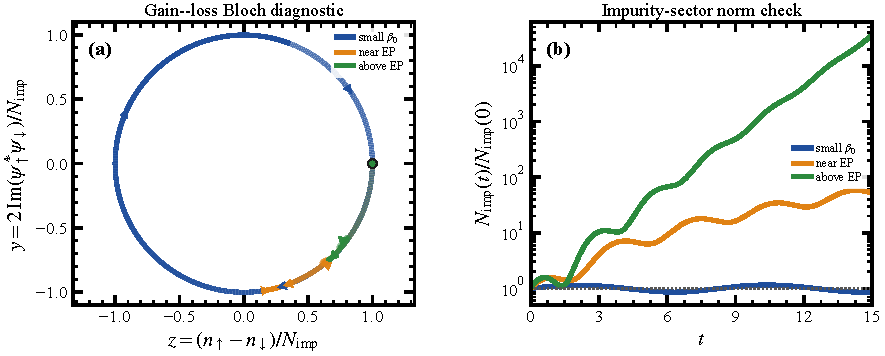
\includegraphics[width=0.92\textwidth]{SFig1_bloch_diagnostic.pdf}
\caption{%
\textbf{Gain--loss Bloch diagnostic for the impurity sector.}
Panel (a) shows the normalized $(z,y)$ trajectory for representative values of
$\beta_0$ below, near, and above the EP.  Below the EP the normalized co-decaying trajectory remains close to the
unbroken relative-kernel orbit, while close to and beyond the EP the trajectory
is progressively distorted.  Panel (b) tracks the impurity-sector norm
$N_{\rm imp}(t)/N_{\rm imp}(0)$ and shows that the above-EP trajectory acquires a
strong late-time amplification, whereas the below-EP and near-EP traces remain
well controlled over the plotted time window.
}
\label{fig:S_bloch}
\end{figure*}

\begin{figure*}[p]
\centering
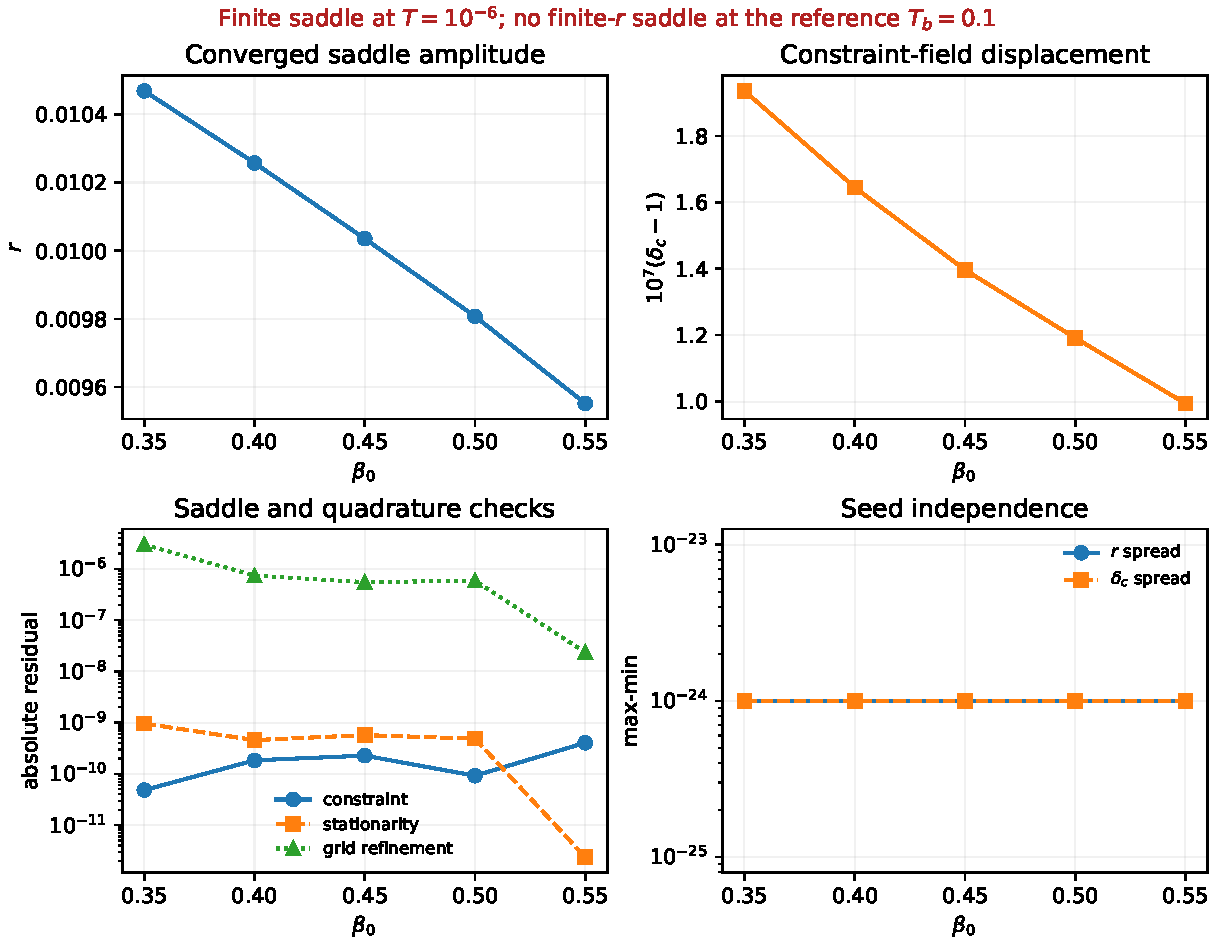
\includegraphics[width=0.92\textwidth]{SFig2_lowT_saddle.pdf}
\caption{%
\textbf{Low-temperature $U\to\infty$ saddle and numerical acceptance tests.}
At $T_{\rm b}=10^{-6}$, panel (a) shows the converged amplitude $r$ and
panel (b) the constraint-field displacement over
$0.35\leq\beta_0\leq0.55$.  Panel (c) reports the final constraint,
stationarity, and grid-refinement residuals; panel (d) shows that real,
negative-real, and complex initial boson seeds converge to the same
gauge-fixed solution.  The complete sandwich construction satisfies charge
continuity to $3.94\times10^{-23}$.  The title records the distinct result at
the manuscript reference temperature: the same closure has no finite-$r$
branch at $T_{\rm b}=0.1$.  The figure therefore validates the low-temperature
saddle and the exact core-EP scaling, but does not claim finite-temperature
condensate enhancement.
}
\label{fig:S_lowT_saddle}
\end{figure*}

\begin{figure*}[p]
\centering

\includegraphics[width=0.92\textwidth]{SFig3_supplemental_diagnostics.pdf}
\caption{%
\textbf{Biorthogonal-projector and finite-$U$ resolvent checks.}
Panel (a) shows the growth of an individual normalized projector and the
artificial $1/s$ factor on the pre-EP side.  Panel (b) verifies numerically
that the two-projector pole sum equals the direct matrix resolvent and that
the two virtual charge sectors equal the closed Schrieffer--Wolff resolvent;
the plotted discrepancies are numerical roundoff.  Panel (c) shows the
complete particle--hole charge factor normalized to its EP limit.  It remains
finite and approaches unity although each projector grows.  These checks
exclude an independent Petermann or $Z^{\rm bio}$ multiplier from the Green
function and screening estimate.
}
\label{fig:S_peakgap}
\end{figure*}

\begin{figure*}[p]
\centering
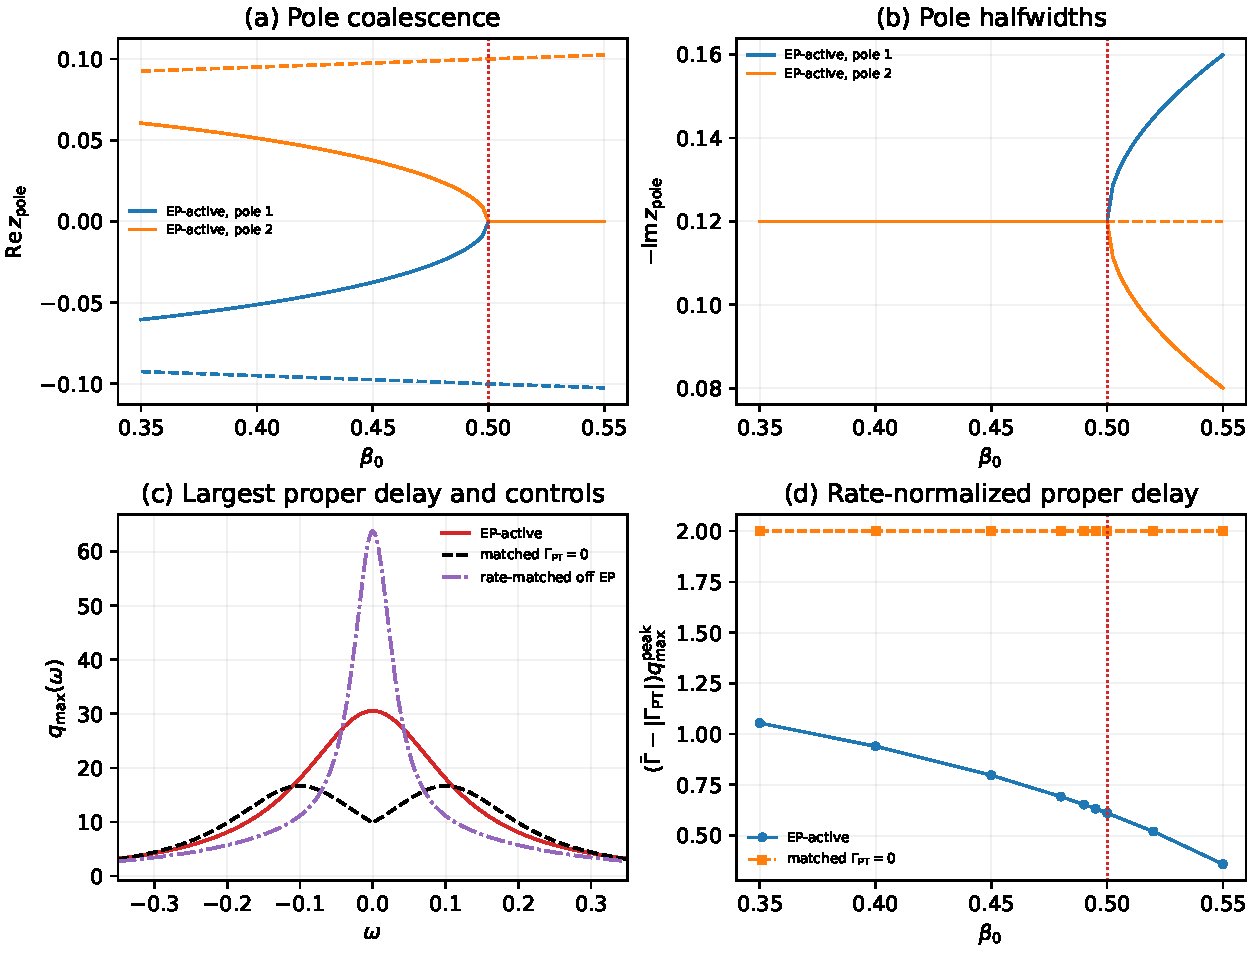
\includegraphics[width=0.92\textwidth]{SFig4_channel_RG.pdf}
\caption{%
\textbf{Causal Smith-delay validation and adverse controls.}
Panel (a) tracks the analytic pole pair to the exact core EP at
$\beta_0=0.50$.  Panel (b) shows the two passive halfwidths: they remain
positive throughout the retained window and split only on the relative-broken
side.  Panel (c) compares the largest proper-delay peak with a Hermitian
control matched by total rate and with an off-EP rate-matched kernel
($D=0.05$); the latter exceeds the EP peak.  Panel (d) normalizes the largest
proper delay by the slowest rate and likewise shows no independent EP
enhancement.  Together with the unitarity and trace-delay checks in
App.~\ref{app:smith}, these controls establish the Smith profile as a causal
coalescence/linewidth fingerprint, not a Kondo-scale multiplier.
}
\label{fig:S_smith}
\end{figure*}

\begin{figure*}[p]
\centering

\includegraphics[width=0.92\textwidth]{SFig4_negative_onset_broadening_check.pdf}
\caption{%
\textbf{Onset of negative signed spectral weight only beyond the EP.}
Panel (a) compares the signed impurity spectral response below the EP
($\beta_0=0.45$), at the EP ($\beta_0=0.50$), and above the EP
($\beta_0=0.58$) for $\delta_{\rm br}=0.015$.  No negative signed relative-kernel response appears below the EP, while
a sign defect emerges only on the PT-broken side.  Panel (b) quantifies the
integrated negative weight $\mathcal W^-$ for
$\delta_{\rm br}=0.014,\,0.015,\,0.020$ and shows that it
remains zero up to the EP and turns on only after
$\beta_{0,{\rm core}}^{\rm EP}=0.50$.
This confirms that the negative signed response is an above-EP effect rather
than a broadening artefact.
}
\label{fig:S_negative_onset}
\end{figure*}

\begin{figure*}[p]
\centering

\includegraphics[width=0.92\textwidth]{Fig3.pdf}
\caption{%
\textbf{Causal scattering and channel-resolved RG support.}
The conservative fixed-$W$ validation uses the complete positive channel
density from $G^R$ and $G^A$, with $\Gamma_0=0.12$ and unit charge gap.
Panel (a) compares the largest causal channel-density eigenvalue at
$\beta_0=0.50$ with the matched $\Gamma_{\rm PT}=0$ control.
Panel (b) gives the Wigner--Smith trace; the passive Fisher--Lee matrix is
unitary to $1.33\times10^{-15}$ and
$\operatorname{Tr}Q(0)=4/\Gamma_0=33.3333$ at the EP.
Panels (c) and (d) show that the EP-active exchange eigenvalue is initially
larger, but its threshold-scale ratio crosses below the control before strong
coupling.  This supports bounded pre-EP weak-flow amplification, not an
enhanced thermodynamic Kondo temperature.
}
\label{fig:S_causal_rg}
\end{figure*}

\begin{figure*}[p]
\centering

\includegraphics[width=0.92\textwidth]{Fig4.pdf}
\caption{%
\textbf{Bath-controlled fluctuation--dissipation and spectral checks.}
The uniform reference is $\epsilon_\xi=-U/2=-1$, $U=2$, and
$T_{\rm b}=0.1$.  Panels (a) and (b) verify the physical construction
$G^<_{\rm phys}=G^R\Sigma^<_{\rm bath}G^A
=f_{\rm FD}(G^A-G^R)$ with maximum residual
$5.61\times10^{-14}$ at $\delta_{\rm br,FDR}=10^{-3}$.
Panel (c) displays the distinct eigenmode occupation ratio only as a
nonnormality diagnostic; it is not used in the saddle equations.
Panel (d) shows the physical impurity spectral response with
$\delta_{\rm br}=0.015$.  Any negative signed response in the broken
relative-kernel continuation is classified as a causality diagnostic rather
than a positive density of states.
}
\label{fig:S_FDR}
\end{figure*}

\begin{figure*}[p]
\centering
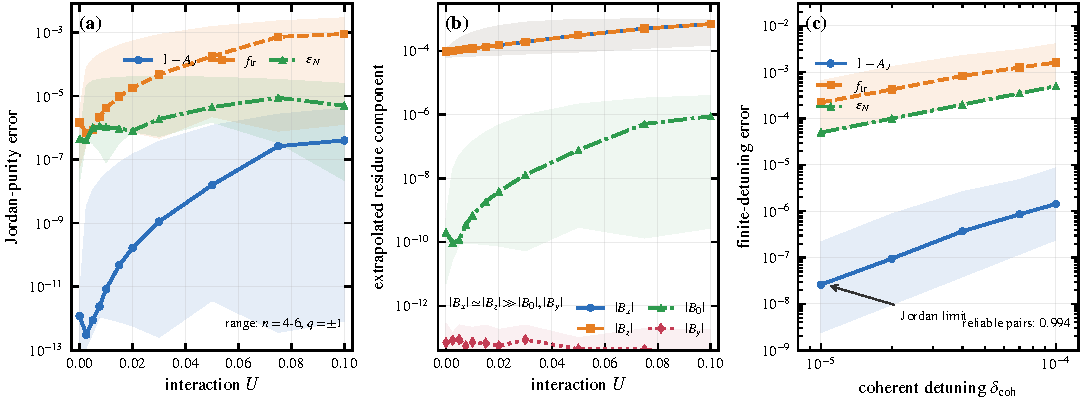
\includegraphics[width=0.98\textwidth]{Fig_NRG_Jordan_structural_clean.pdf}
\caption{%
\textbf{Finite-$U$ Jordan transition-residue audit for the
scalar-hybridization NRG control.}
(a) Zero-detuning extrapolations of the alignment error $1-A_J$, trace
fraction $f_{\rm tr}$, and nilpotent mismatch $\epsilon_N$.  Curves are
medians and bands are the full range over iterations $n=4$--$6$ and charge
sectors $q=\pm1$.  (b) Pauli components of the extrapolated double-pole
coefficient $B$: $|B_x|\simeq|B_z|\gg|B_0|,|B_y|$, as required by
$N_{\rm EP}=\Deff\sigma_z+i\Gpt\sigma_x$.  (c) Direct finite-detuning
convergence; curves are medians and bands are the 16th--84th percentile over
$U$, iteration, and tracked sector.  The reliable-pair fraction is $0.994$.
Parameters are $\Lambda=3$, $z=0.5$, $N_{\rm keep}=320$, $r=1$,
$\beta_0=0.50$, $\Deff=\Gpt=0.10$, and $0\leq U\leq0.10$.  The figure
establishes persistence of the nilpotent matrix-residue direction; it does
not establish pole coalescence, a universal interaction law, a thermodynamic
Kondo scale, or a phase boundary.
}
\label{fig:S_NRG_Jordan}
\end{figure*}

\clearpage

\section*{Reproducibility}
The numerical scripts, parameter tables, and exported data used for the main
and Supplemental figures are included in the accompanying archive and in the
version-controlled GitHub repository
\href{https://github.com/VMKPHYSMATH/emergent-pt-dirac-impurity}{\texttt{VMKPHYSMATH/emergent-pt-dirac-impurity}}~\cite{kulkarni2026code}.
Release v1.0.1 is archived at
\href{https://doi.org/10.5281/zenodo.21434683}{doi:10.5281/zenodo.21434683};
the all-versions record is
\href{https://doi.org/10.5281/zenodo.21434682}{doi:10.5281/zenodo.21434682}.
The accompanying source also includes
\nolinkurl{verify_finiteU_contact_algebra.py}, which reproduces the
finite-\(U\) \(R\)-matrix, CPT-covariance, and YBE residuals quoted above.
The NRG archive additionally contains the independent transition-operator
propagation, no-truncation regression, branch-tracking and convergence
scripts, the gate summary, and the exported data used in
Fig.~\ref{fig:S_NRG_Jordan}.

\bibliography{ref}

\end{document}
